\documentclass[xcolor={table}]{beamer}
\usepackage{fleqn}
%\usepackage{epsf}
\usepackage{graphicx}
\usepackage{coordsys} %for \numbline command
%\usepackage{dingbat}
%\usepackage{aima2e-slides}

%Setup appearance:

\usetheme{Darmstadt}
% Hunting Errors
%\usefonttheme[onlylarge]{structurebold}
\usefonttheme{professionalfonts} %this ensures beamer doesn't mess up the \hat and \tilde commands

\setbeamerfont*{frametitle}{size=\normalsize,series=\bfseries}
\setbeamertemplate{navigation symbols}{}
\setbeamertemplate{bibliography item}{[\theenumiv]}
\setbeamertemplate{caption}[numbered]

% Standard packages
% Hunting Errors
%\usepackage[english]{babel}
\usepackage[latin1]{inputenc}
\usepackage{times}
\usepackage[T1]{fontenc}
\usepackage{multirow}
\usepackage{subfigure}
\usepackage{pbox}
\usepackage{arydshln}
\usepackage{pifont}
\usepackage{cancel}

% Source Code packages
%\usepackage{algorithmicx}
\usepackage{algorithm}
\usepackage{algpseudocode}
\algrenewcommand\alglinenumber[1]{\tiny #1:} %make the line number size in the algorithmicx algorithm environment (which is loaded by algpseudocode smaller
%\algsetup{linenosize=\tiny}
%\usepackage{algorithm2e}

% Hunting Errors
\usepackage{listings}
\lstset{ %
language=Octave,                % choose the language of the code
basicstyle=\footnotesize,       % the size of the fonts that are used for the code
numbers=left,                   % where to put the line-numbers
numberstyle=\footnotesize,      % the size of the fonts that are used for the line-numbers
stepnumber=1,                   % the step between two line-numbers. If it's 1 each line will be numbered
numbersep=5pt,                  % how far the line-numbers are from the code
backgroundcolor=\color{white},  % choose the background color. You must add \usepackage{color}
showspaces=false,               % show spaces adding particular underscores
showstringspaces=false,         % underline spaces within strings
showtabs=false,                 % show tabs within strings adding particular underscores
frame=single,	                % adds a frame around the code
tabsize=2,	                % sets default tabsize to 2 spaces
captionpos=b,                   % sets the caption-position to bottom
breaklines=true,                % sets automatic line breaking
breakatwhitespace=false,        % sets if automatic breaks should only happen at whitespace
escapeinside={\%*}{*)}          % if you want to add a comment within your code
}



% to correct indentation in algorithmic environments
% https://www.latex4technics.com/?note=wwr
%\newcommand{\algmargin}{\the\ALG@thistlm}
%\makeatother
%\newlength{\whilewidth}
%\settowidth{\whilewidth}{\algorithmicwhile\ }
%\algdef{SE}[parWHILE]{parWhile}{EndparWhile}[1]
%  {\parbox[t]{\dimexpr\linewidth-\algmargin}{%
%     \hangindent\whilewidth\strut\algorithmicwhile\ #1\ \algorithmicdo\strut}}{\algorithmicend\ \algorithmicwhile}
%\algnewcommand{\parState}[1]{\State%
%  \parbox[t]{\dimexpr\linewidth-\algmargin}{\strut #1\strut}}

% Setup TikZ
\usepackage{tikz}
\usetikzlibrary{arrows}
\tikzstyle{block}=[draw opacity=0.7,line width=1.4cm]

%%%%%%%%%%%%%%%%%%%%%%%%%%%%%%%%%%%%%%%%%%%%
%% Start newcommand defs taken from aima slides style file %%%%%%%%%%%%%%
%%%%%%%%%%%%%%%%%%%%%%%%%%%%%%%%%%%%%%%%%%%%

%%%%%%%%%%%% elements of programs %%%%%%%%%%%%%%%%%%%%%%%%%%%%%%%%%


\newlength{\codewidth}
\setlength{\codewidth}{\textwidth}
\addtolength{\codewidth}{-0.5in}

\newcommand{\FigBox}[1]{%%% The alternative to figbox - pnorvig
\noindent\framebox[\textwidth]{%
\begin{minipage}{\codewidth}%
#1%
\end{minipage}}%
}

\newcommand{\defprog}[1]{\txr{\mbox{{\sc #1}}}}
\newcommand{\prog}[1]{\mbox{{\sc #1}}}   %%% same as defprog
\newcommand{\noprog}[1]{\mbox{{\sc #1}}} %%% same as defprog
\newcommand{\system}[1]{\mbox{{\sc #1}}} %%% same as defprog
\newcommand{\nosystem}[1]{\mbox{{\sc #1}}} %%% same as defprog
\newcommand{\act}[1]{{\it #1}}
\newcommand{\key}[1]{\txb{{\bf #1}}}
\def\k{\key}
\newcommand{\var}[1]{\txg{{\it #1}}}
\def\v{\var}
\def\p{\prg}
\newcommand{\setq}[2]{#1\hbox{$\,\leftarrow\,$}#2}
\newcommand{\setqmath}[2]{#1 \leftarrow #2}

%%pnorvig Mar 14 1994:
\newcommand{\labl}[1]{\prog{#1}}	% Statement Label in code
\newcommand{\cmt}[1]{{\tt /*} {\it #1} {\tt */}}	% Comment in code
\newcommand{\rcmt}[1]{\hfill {\tt /*} {\it #1} {\tt */}}
\newcommand{\Endfn}[1]{}		% End of a function in code
\newcommand{\fnsep}{\hspace*{0in}\raisebox{3pt}{\rule{\codewidth}{0.2pt}}\hfill}	% Between functions in code

\def\code{\noindent\nobreak\begin{scriptsize}
        \begingroup\obeylines\obeyspaces\docode}
\def\docode#1{\noindent\framebox[\columnwidth][l]%
{~~\begin{minipage}{\codewidth}~
#1
~\end{minipage}}\endgroup%
\nobreak\end{scriptsize}\noindent\ignorespaces}
\def\asis{\obeylines\obeyspaces}
\def\ttp{.\skip -0.5em\ }
{\obeyspaces\global\def {\ }}

%% Fine tuning for perfect formatting

\newcommand{\ac}{,\hspace{0.15em}}
\newcommand{\ts}{\,}
\newcommand{\bodysep}{\vspace{0.1in}}
\newcommand{\subfnsep}{\vspace{0.06in}}
\newcommand{\prebnfsep}{\vspace{-0.25in}}
\newcommand{\postbnfsep}{\vspace{0.1in}}
\newcommand{\fnvar}[1]{\prog{#1}}
\newcommand{\func}[3]{\key{function} \defprog{#1}(\txg{#2}) \key{returns} #3}
\newcommand{\nofunc}[3]{\key{function} \noprog{#1}(#2) \key{returns} #3}
\newcommand{\proc}[2]{\key{procedure} \defprog{#1}(\txg{#2})}
\newcommand{\noproc}[2]{\key{procedure} \noprog{#1}(#2)}
\newcommand{\firstinputs}[2]{\key{inputs}: \var{#1}, #2}
\newcommand{\inputs}[2]{\phantom{\key{inputs}: }\var{#1}, #2}
\newcommand{\firstlocal}[2]{\key{local variables}: \var{#1}, #2}
\newcommand{\local}[2]{\phantom{\key{local variables}: }\var{#1}, #2}
\newcommand{\firststatic}[2]{\key{static}: \var{#1}, #2}
\newcommand{\static}[2]{\phantom{\key{static}: }\var{#1}, #2}

%%%%%%%%%%%%%%%%%%%%%%%%%%

\def\mysum{\begin{Huge}\mbox{$\Sigma$}\end{Huge}}
\def\myint{\begin{LARGE}\mbox{$\int$}\end{LARGE}}
\def\myprod{\begin{Huge}\mbox{$\Pi$}\end{Huge}}

\font\smathbold=cmbx10 scaled 1700
\newcommand{\smbf}[1]{\mbox{{\smathbold #1}}}
\newcommand{\mbf}[1]{\mbox{{\bf #1}}}

%%%%%%% Useful formatting commands for lines of text etc.
\def\tab{\hbox{\kern0.4in}}    %% Insert space (even at start of line)
\def\al{\\\tab}                %% Next line is indented
\def\nl{\\\tab\tab}            %% Next line is double-indented
\def\nnl{\\\tab\tab\tab}       %% Next line is triple-indented
%\def{$\diamondsuit\ \ $}  %% Itemization without all the spacing
\def\bull{\vskip -8pt\item{$\bullet$\ }} %% Itemization with less spacing
\def\u#1{$\underline{\mbox{#1}}$}
\def\q#1{\txm{\u{#1}??}}

%%%%%% logical symbols
\newcommand{\entails}{\models}
%\newcommand{\implies}{\:\;{\Rightarrow}\:\;}
\newcommand{\textimplies}{\;{\Rightarrow}\;}
\newcommand{\impliessymbol}{\Rightarrow}
\newcommand{\lequiv}{\;\;{\Leftrightarrow}\;\;}
\newcommand{\textlequiv}{\;{\Leftrightarrow}\;}
\newcommand{\lequivsymbol}{\Leftrightarrow}
\newcommand{\xor}{\not\lequiv}
\newcommand{\All}[1]{\forall\,#1\;\;}
\newcommand{\Exi}[1]{\exists\,#1\;\;}
\newcommand{\Exii}[1]{\exists!\,#1\;\;}% -pnorvig
\newcommand{\Iot}[2]{\iota\,#1\,#2}
\newcommand{\Lam}[2]{\lambda #1\;#2}
\newcommand{\Qua}[3]{[#1\,#2\;#3]}

\newcommand{\union}{{\,{\cup}\,}}
\newcommand{\intersection}{{\,{\cap}\,}}
\renewcommand{\emptyset}{\{\,\}}
\newcommand{\emptylist}{[\,]}
\newcommand{\adjoin}[2]{\{#1|#2\}}
\newcommand{\elt}{{\,{\in}\,}}  %%%cuts down on spacing
\newcommand{\eq}{{\,{=}\,}}  %%%cuts down on spacing
\def\stimes{{\,\times\,}}       %%%cuts down on spacing


%%%%%%% Formatting tables - AIMA uses full-width tables with spacing

\newenvironment{mytabular}%
{\noindent\begin{tabular*}{\textwidth}}%
{\end{tabular*}}

\newcommand{\tabtop}{\rule{0pt}{2ex}}%%Use after hline in body of table
\newcommand{\tabbot}{\rule[-1ex]{0pt}{1.8ex}}%%Use before hline " " " "
\newcommand{\tabhead}{\rule[-0.85ex]{0pt}{2.8ex}}%%Use in lines between hlines
\newcommand{\squad}{\hspace*{0.5em}}%%Use occasionally at left edge
\newcommand{\sq}[1]{\hspace*{#1\textwidth}}
\def\tf{\rm} %% table font


\def\<{\langle}
\def\>{\rangle}

%\usepackage[dvips]{color}
\definecolor{myred}{rgb}{0.7,0.0,0.0}
\definecolor{myblue}{rgb}{0.0,0.0,0.5}
\definecolor{mygreen}{rgb}{0.0,0.3,0.0}

\newcommand{\txr}[1]{\textcolor{myred}{#1}}
\newcommand{\txR}[1]{\textcolor{red}{#1}}
\newcommand{\txb}[1]{\textcolor{myblue}{#1}}
\newcommand{\txg}[1]{\textcolor{mygreen}{#1}}
\newcommand{\txm}[1]{\textcolor{magenta}{#1}}

\newcommand{\mat}[1]{\textcolor{myred}{#1}}
\newcommand{\defn}[1]{\textcolor{myblue}{#1}}
\newcommand{\mynote}[1]{\textcolor{mygreen}{#1}}


\newcommand{\sr}[1]{\mathrel{\raisebox{-0.6ex}{$\stackrel{#1}{\longrightarrow}$}}}
\newcommand{\srbox}[1]{\sr{\fboxsep=1pt\fbox{$\,{\scriptstyle #1}\,$}}}
\newcommand{\srboxbox}[1]{\sr{\fboxsep=1pt\fbox{\fbox{$\,{\scriptstyle #1}\,$}}}}

\def\Diff{\mbox{{\it Diff}}}

%%%%%% probability and decision theory
\newcommand{\pv}{\mbf{P}}
\newcommand{\qv}{\mbf{Q}}
\newcommand{\given}{\mid}
\def\transition#1#2{q(#1\rightarrow #2)}
\newcommand{\otherthan}{\overline}
\newcommand{\Parents}{Parents}
\newcommand{\parents}{parents}
\newcommand{\Children}{Children}
\newcommand{\children}{children}
\newcommand{\MarkovBlanket}{MB}
\newcommand{\markovBlanket}{mb}


\def\X{\mbf{X}}
\def\x{\mbf{x}}
\def\sx{\smbf{x}}
\def\Y{\mbf{Y}}
\def\y{\mbf{y}}
\def\sy{\smbf{y}}
\def\E{\mbf{E}}
\def\e{\mbf{e}}
\def\D{\mbf{D}}
\def\d{\mbf{d}}
\def\sbe{\smbf{e}}
\def\sE{\smbf{E}}
\def\T{\mbf{T}}
\def\O{\mbf{O}}
\def\se{\smbf{e}}
\def\Z{\mbf{Z}}
\def\z{\mbf{z}}
\def\sz{\smbf{z}}
\def\F{\mbf{F}}
\def\f{\mbf{f}}
\def\A{\mbf{A}}
\def\B{\mbf{B}}
\def\C{\mbf{C}}
\def\b{\mbf{b}}
\def\m{\mbf{m}}
\def\I{\mbf{I}}
\def\H{\mbf{H}}
\def\zeroes{\mbf{0}}
\def\ones{\mbf{1}}
\def\ev{\mbf{ev}}
\def\fv{\mbf{ev}}
\def\sv{\mbf{sv}}

\usepackage{rotating} % for sideways headings

%\usepackage{listings}
%\usepackage{xfrac} % for slanted fractions using sfrac
%
%% the answer environment
%\usepackage{verbatim}   % for the comment environment
%\usepackage{ifthen}
%\usepackage{lipsum}
%\newenvironment{answer}%
%        {%
%            \ifthenelse{\isundefined{\showanswer}}%
%                    {\expandafter\comment}%
%                    {~\\ \noindent\rule{\textwidth}{0.4pt}}%
%                    }%
%         {%
%            \ifthenelse{\isundefined{\showanswer}}%
%                    {\expandafter\endcomment}%
%                    {~\\ \noindent\rule{\textwidth}{0.4pt} \newpage}%
%          }
%
%\usepackage{arydshln}
%\usepackage{capt-of}

\DeclareSymbolFont{extraup}{U}{zavm}{m}{n}
\DeclareMathSymbol{\varclub}{\mathalpha}{extraup}{84}
\DeclareMathSymbol{\varspade}{\mathalpha}{extraup}{85}
\DeclareMathSymbol{\varheart}{\mathalpha}{extraup}{86}
\DeclareMathSymbol{\vardiamond}{\mathalpha}{extraup}{87}

%%%%%%%%%%%%%%%%%%%%%%%%%%%%%%%%%%%%%%%%%%%%
%% End newcommand defs taken from aima slides style file %%%%%%%%%%%%%%
%%%%%%%%%%%%%%%%%%%%%%%%%%%%%%%%%%%%%%%%%%%%

\usepackage{xifthen}% provides \isempty test
\newcommand{\SectionSlide}[2][]{
	\ifthenelse{\isempty{#1}}
		{\section{#2}\begin{frame} \begin{center}\begin{huge}#2\end{huge}\end{center}\end{frame}}
		{\section[#1]{#2}\begin{frame} \begin{center}\begin{huge}#2\end{huge}\end{center}\end{frame}}
}
\urlstyle{same} %ensure that urls are formatted in the same font as other text

% tikz sert up for MDP diagrams
%\usepackage{tikz}			% for MDP dfiagrams
%\usetikzlibrary{positioning,angles,quotes}
\usepackage{pgfplots}         % it load tikz too
%\pgfplotsset{compat=1.16}
\pgfplotsset{compat=1.14}
\usetikzlibrary{automata,
                arrows.meta,    %   ...customizing arrows
                positioning,    %   ...positioning nodes
                quotes}         % For edge labels
\usepgfplotslibrary{fillbetween}


%To get Table, Figure, Equation Numbers to work!
\usepackage{xr}
\externaldocument{FMLPDA2-Main-NewMathTemplate}
%To get nice labeled matrices in  MDB examples
%\usepackage{kbordermatrix}
 % For vertical alignment in table cells
\usepackage[export]{adjustbox}
% For citet and citep commands
\usepackage[round]{natbib}

%Use tikz package and command is used to put circles around symbols inline useful for NN examples
\newcommand*\circled[1]{\tikz[baseline=(char.base)]{
            \node[shape=circle,draw,inner sep=2pt,minimum size=20pt] (char) {#1};}}

\newcommand{\Toprule}[0]{\hline}
\newcommand{\Midrule}[0]{\hline}
\newcommand{\Botrule}[0]{\hline}
\DeclareMathOperator*{\argmax}{arg\,max}
\DeclareMathOperator*{\argmin}{arg\,min}

\newcommand{\keyword}[1]{{\textbf{#1}}\index{#1}}
\newcommand{\indexkeyword}[1]{#1\index{#1}}
\newcommand{\keywordDef}[1]{{\textbf{#1}}\index{#1|textbf}}
\newcommand{\indexkeywordDef}[1]{{#1}\index{#1|textbf}}
\newcommand{\keywordAlias}[2]{{\textbf{#1}}\index{#2}}
\newcommand{\indexkeywordAlias}[2]{#1\index{#2}}
\newcommand{\keywordDefAlias}[2]{{\textbf{#1}}\index{#2|textbf}}
\newcommand{\indexkeywordDefAlias}[2]{{#1}\index{#2|textbf}}
\newcommand{\keywordCR}[2]{{\textbf{#1}}\index{#1|see {#2}}}
\newcommand{\keywordCRAlias}[3]{{\textbf{#1}}\index{#2|see {#3}}}
\newcommand{\indexkeywordCR}[2]{#1\index{#1|see {#2}}}
\newcommand{\indexkeywordCRAlias}[3]{#1\index{#2|see {#3}}}
\newcommand{\mightdo}[1]{}
\newcommand{\featN}[1]{\textsc{#1}}
\newcommand{\featL}[1]{\textit{#1}}
 \newcommand{\ourRef}[1]{\ref{#1}$^{\text{\tiny[\pageref{#1}]}}$}
 \newcommand{\ourEqRef}[1]{\eqref{#1}$^{\text{\tiny[\pageref{#1}]}}$}
 \newcommand{\ourItemExtra}{\item[\raisebox{0.25ex}{$\mathbf{\Asterisk}$} \addtocounter{enumi}{1}\arabic{enumi}.]} 
 \newcommand{\rlState}[1]{\textsc{#1}} % Used in reinforcement learning chapter
\newcommand{\rlAction}[1]{\textit{#1}} % Used in reinforcement learning chapter



\title{Beyond Prediction: Unsupervised Learning}
	\author{John D. Kelleher and Brian Mac Namee and Aoife D'Arcy}
	\institute{}
	\date{}
\begin{document}
\begin{frame}
	\titlepage
\end{frame}
\begin{frame}
	 \tableofcontents[hideallsubsections]
%	 \tableofcontents
\end{frame}
\SectionSlide{Big Idea}



 \begin{frame} 
\begin{figure}[htb]
       \begin{centering}
			\subfigure[The fridge]{\includegraphics[width=0.22\textwidth]{images/fmlpda_figure_10_1_a.png}} ~ 
			\subfigure[Abigail]{\includegraphics[width=0.22\textwidth]{images/fmlpda_figure_10_1_b.png}} ~
			\subfigure[Andrew]{\includegraphics[width=0.22\textwidth]{images/fmlpda_figure_10_1_c.png}} ~
			\subfigure[Amalia]{\includegraphics[width=0.22\textwidth]{images/fmlpda_figure_10_1_d.png}}
       \caption{The three different arrangements of the magnetic letters made by the Murphy children on the Murphy family refrigerator.}
       \label{fig:fridgeLetters}
       \end{centering}
\end{figure}
\end{frame} 


\SectionSlide{Fundamentals}



 \begin{frame} 
\begin{figure}[htb]
       \begin{centering}
       \includegraphics[width=0.7\textwidth]{images/fmlpda_figure_10_2.pdf}
       \caption{Unsupervised machine learning as a single-step process.}
       \label{fig:unsupervisedlearning}
       \end{centering}
\end{figure}
\end{frame} 


\SectionSlide{Standard Approach: The $k$-Means Clustering Algorithm}



 \begin{frame} 
\begin{equation}
\sum_{i=1}^n \min_{{\mathbf{c}_1},\ldots, {\mathbf{c}_k}} {Dist}(\mathbf{d}_i, {\mathbf{c}_j})
\end{equation}
\end{frame} 



\begin{frame}[plain]
\scriptsize{Pseudocode description of the \keywordAlias{\textit{k}-means clustering}{k-means clustering} algorithm.}
\begin{footnotesize}
%\begin{algorithm}[htb]
%\caption{Pseudocode description of the \keywordAlias{\textit{k}-means clustering}{k-means clustering} algorithm.}
%\label{alg:kmeans}
\begin{algorithmic}[1]
\Require a dataset $\mathcal{D}$ containing $n$ training instances, $\mathbf{d}_1, \ldots, \mathbf{d}_n$ 
\Require the number of clusters to find $k$
\Require a distance measure, ${Dist}$, to compare instances to cluster centroids
\State Select $k$ random cluster centroids, ${\mathbf{c}_1}$ to ${\mathbf{c}_k}$, each defined by values for each descriptive feature, $\mathbf{c}_i = <\mathbf{c}_i[1], \dots, \mathbf{c}_i[m]>$
\Repeat
\State{calculate the distance of each instance, $\mathbf{d}_i$, to each cluster centroid, ${\mathbf{c}_1}$ to ${\mathbf{c}_k}$, using ${Dist}$}
\State{assign each instance, $\mathbf{d}_i$, to belong to the cluster, $\mathcal{C}_i$, to whose cluster centroid, ${\mathbf{c}_i}$, it is closest}
\State{update each cluster centroid, ${\mathbf{c}_i}$, to the average of the descriptive feature values of the instances that belong to cluster $\mathcal{C}_i$}
\Until{no cluster reassignments are performed during an iteration} 
\end{algorithmic}
%\end{algorithm}
\end{footnotesize}
\end{frame}



\subsection{A Worked Example}

\begin{frame}[plain]
\begin{table}[!tbh]
%\begin{table}[!tbh]
\caption{A dataset of mobile phone customers described by their average monthly data (\featN{Data Usage}) and call (\featN{Call Volume}) usage. Details of the first two iterations of the \textit{k}-means clustering algorithm are also shown. }
\label{table:kmeansDemoData}
\begin{tiny}
{\setlength{\tabcolsep}{0.6em}
\begin{tabular*}{\textwidth}{@{\extracolsep{\fill}} rrr | rrrc | rrrc @{}}
\Toprule
~	 & \featN{Data} & \featN{Call} & \multicolumn{3}{c}{Cluster Distances Iter. 1} & Iter. 1  & \multicolumn{3}{c}{Cluster Distances Iter. 2} & Iter. 2\\
\featN{ID}	 & \featN{Usage} & \featN{Volume} & ${Dist}(\mathbf{d}_i, {\mathbf{c}_1})$ & ${Dist}(\mathbf{d}_i, {\mathbf{c}_2})$ & ${Dist}(\mathbf{d}_i, {\mathbf{c}_3})$ & Cluster & ${Dist}(\mathbf{d}_i, {\mathbf{c}_1})$ & ${Dist}(\mathbf{d}_i, {\mathbf{c}_2})$ & ${Dist}(\mathbf{d}_i, {\mathbf{c}_3})$ & Cluster\\
\Midrule
1 & -0.9531 & -0.3107 & 0.2341 & 0.9198 & 0.6193 & $\mathcal{C}_1$ & 0.4498 & 1.9014 & 1.1099 & $\mathcal{C}_1$ \\ 
2 & -1.1670 & -0.7060 & 0.5770 & 0.6108 & 0.9309 & $\mathcal{C}_1$ & 0.87 & 2.0554 & 1.558 & $\mathcal{C}_1$ \\ 
3 & -1.2329 & -0.4188 & 0.3137 & 0.8945 & 0.6388 & $\mathcal{C}_1$ & 0.7464 & 2.152 & 1.3661 & $\mathcal{C}_1$ \\ 
4 & 1.0684 & -0.4560 & 2.1972 & 2.06 & 2.438 & $\mathcal{C}_2$ & 1.6857 & 0.3813 & 1.7651 & $\mathcal{C}_2$ \\ 
5 & -1.1104 & 0.1090 & 0.2415 & 1.3594 & 0.1973 & $\mathcal{C}_3$ & 0.5669 & 2.1905 & 0.923 & $\mathcal{C}_1$ \\ 
6 & -0.8431 & 0.1811 & 0.4084 & 1.405 & 0.4329 & $\mathcal{C}_1$ & 0.3694 & 1.9842 & 0.6651 & $\mathcal{C}_1$ \\ 
7 & -0.3666 & 0.6905 & 1.1055 & 1.9728 & 1.0231 & $\mathcal{C}_3$ & 0.7885 & 1.9406 & 0.0837 & $\mathcal{C}_3$ \\ 
8 & 0.9285 & -0.2168 & 2.0351 & 2.0378 & 2.2455 & $\mathcal{C}_1$ & 1.5083 & 0.5759 & 1.5127 & $\mathcal{C}_2$ \\ 
9 & 1.1175 & -0.6028 & 2.2715 & 2.0566 & 2.529 & $\mathcal{C}_2$ & 1.772 & 0.298 & 1.895 & $\mathcal{C}_2$ \\ 
10 & 0.8404 & -1.0450 & 2.1486 & 1.693 & 2.4636 & $\mathcal{C}_2$ & 1.7165 & 0.258 & 2.0328 & $\mathcal{C}_2$ \\ 
11 & -1.005 & -0.0337 & 0.1404 & 1.2012 & 0.3692 & $\mathcal{C}_1$ & 0.4339 & 2.0376 & 0.9295 & $\mathcal{C}_1$ \\ 
12 & 0.2410 & 0.7360 & 1.6017 & 2.2398 & 1.6013 & $\mathcal{C}_3$ & 1.1457 & 1.6581 & 0.5908 & $\mathcal{C}_3$ \\ 
13 & 0.2021 & 0.4364 & 1.4253 & 1.9619 & 1.4925 & $\mathcal{C}_1$ & 0.9259 & 1.4055 & 0.5668 & $\mathcal{C}_3$ \\ 
14 & 0.2153 & 0.8360 & 1.6372 & 2.3159 & 1.6125 & $\mathcal{C}_3$ & 1.2012 & 1.7602 & 0.5956 & $\mathcal{C}_3$ \\ 
15 & 0.8770 & -0.2459 & 1.985 & 1.9787 & 2.201 & $\mathcal{C}_2$ & 1.4603 & 0.5454 & 1.4865 & $\mathcal{C}_2$ \\ 
16 & -0.0345 & 1.0502 & 1.595 & 2.4136 & 1.4929 & $\mathcal{C}_3$ & 1.2433 & 2.0589 & 0.5321 & $\mathcal{C}_3$ \\ 
17 & 0.8785 & -1.3601 & 2.3325 & 1.727 & 2.6698 & $\mathcal{C}_2$ & 1.9413 & 0.569 & 2.3167 & $\mathcal{C}_2$ \\ 
18 & 0.9164 & -0.8517 & 2.1454 & 1.7984 & 2.4383 & $\mathcal{C}_2$ & 1.6815 & 0.0674 & 1.9271 & $\mathcal{C}_2$ \\ 
19 & -1.0423 & 0.1193 & 0.2593 & 1.3579 & 0.2525 & $\mathcal{C}_3$ & 0.5065 & 2.133 & 0.8608 & $\mathcal{C}_1$ \\ 
20 & -0.7426 & 0.0119 & 0.3899 & 1.2399 & 0.5706 & $\mathcal{C}_1$ & 0.1889 & 1.8164 & 0.7247 & $\mathcal{C}_1$ \\ 
21 & 0.6259 & -1.1834 & 2.0248 & 1.4696 & 2.3616 & $\mathcal{C}_2$ & 1.6355 & 0.4709 & 2.0374 & $\mathcal{C}_2$ \\ 
22 & 0.7684 & -0.5844 & 1.927 & 1.7338 & 2.195 & $\mathcal{C}_2$ & 1.4362 & 0.2382 & 1.6289 & $\mathcal{C}_2$ \\ 
23 & -0.2596 & 0.7450 & 1.2183 & 2.0535 & 1.1432 & $\mathcal{C}_3$ & 0.8736 & 1.9167 & 0.1535 & $\mathcal{C}_3$ \\ 
24 & -0.3414 & 0.4215 & 0.9432 & 1.7202 & 0.9548 & $\mathcal{C}_1$ & 0.5437 & 1.7259 & 0.1909 & $\mathcal{C}_3$ \\ 
\Botrule
\end{tabular*}
}
{}
\end{tiny}
%\end{table}
\end{table}
\end{frame}

 \begin{frame} 
\begin{figure}[!t]
\vspace{-1em}
{\setlength{\tabcolsep}{0.05em}
\begin{tabular}{ccc}

	\subfigure[]{\label{fig:kmeansDemoData}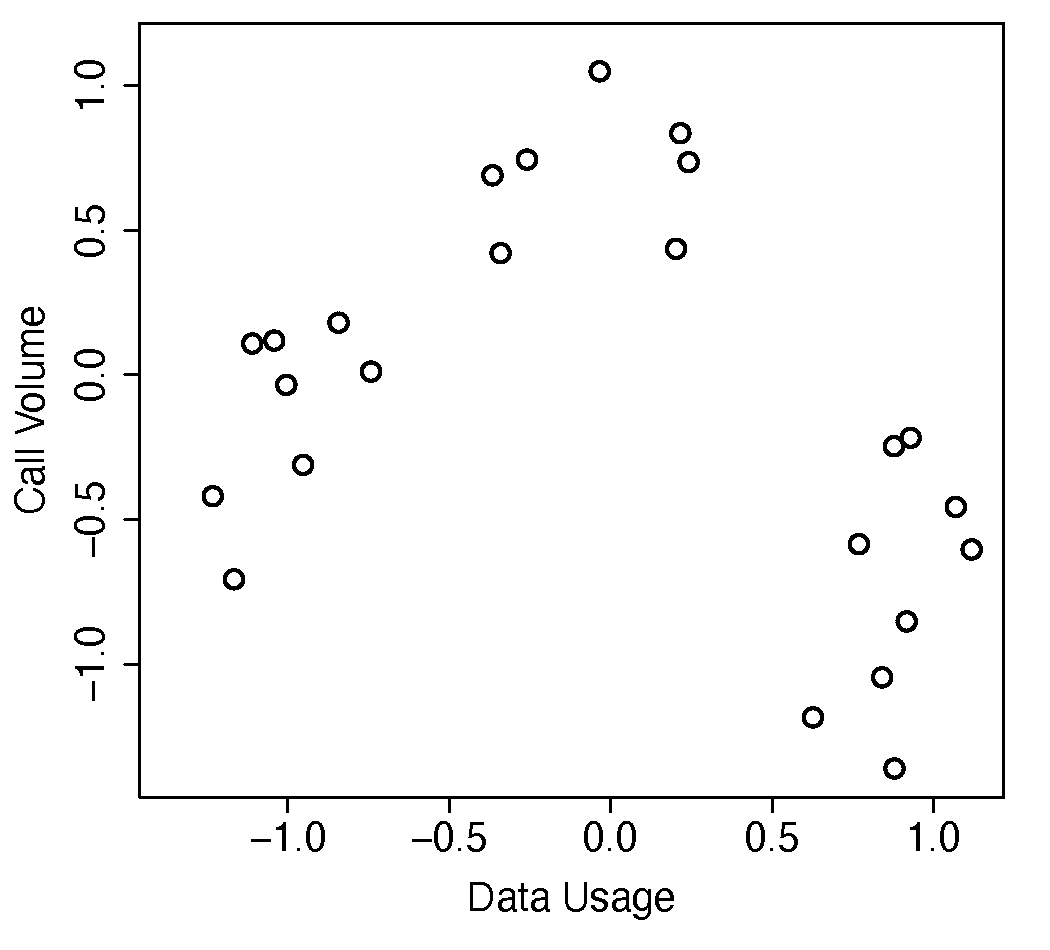
\includegraphics[width=0.22\linewidth]{./images/fmlpda_figure_10_3_a.pdf}}&
	\subfigure[]{\label{fig:kmeansDemo2}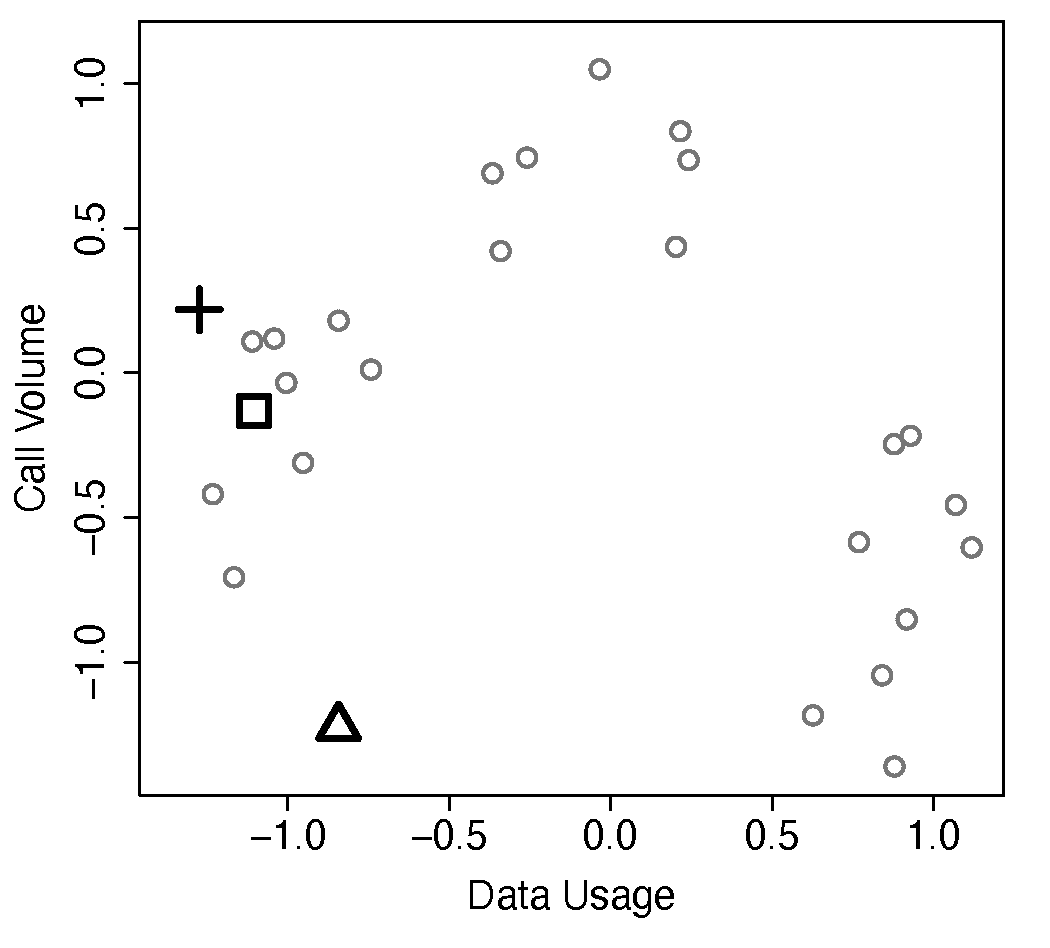
\includegraphics[width=0.22\linewidth]{./images/fmlpda_figure_10_3_b.pdf}}&
	\subfigure[]{\label{fig:kmeansDemo3}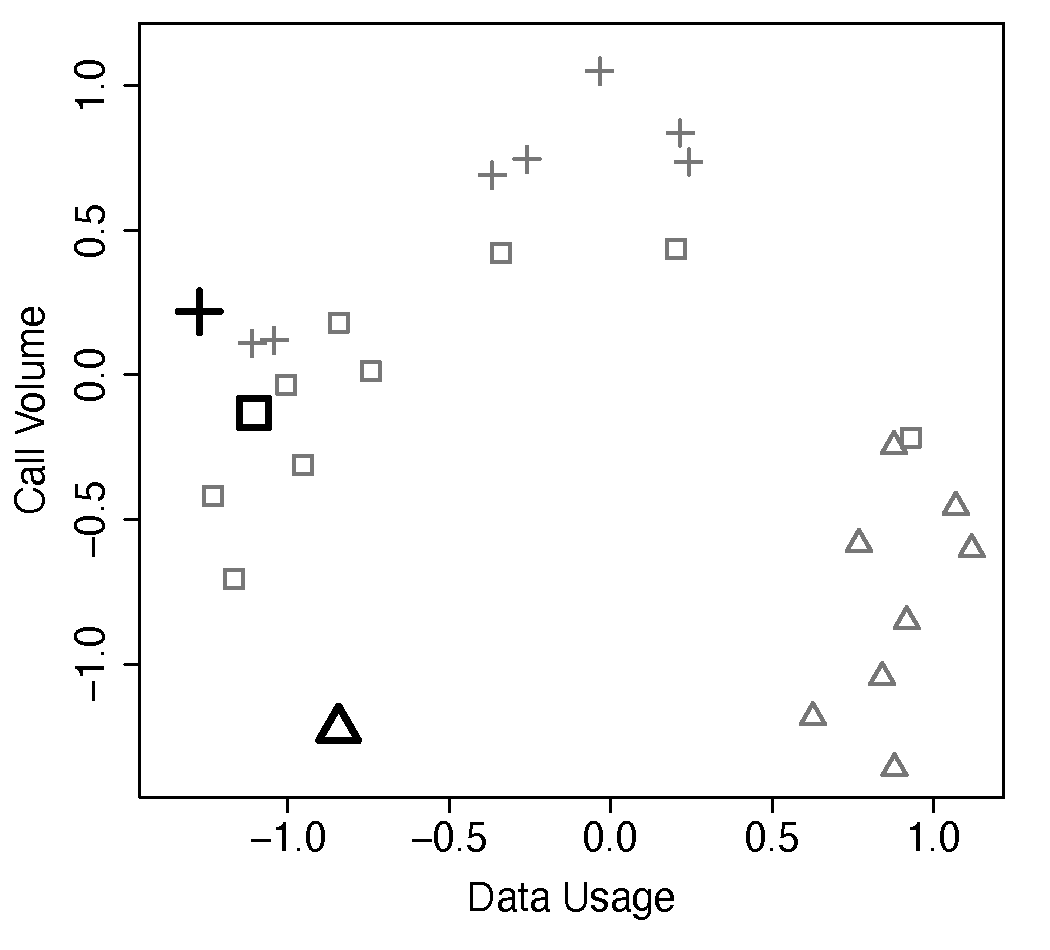
\includegraphics[width=0.22\linewidth]{./images/fmlpda_figure_10_3_c.pdf}} \\

	\subfigure[]{\label{fig:kmeansDemo4}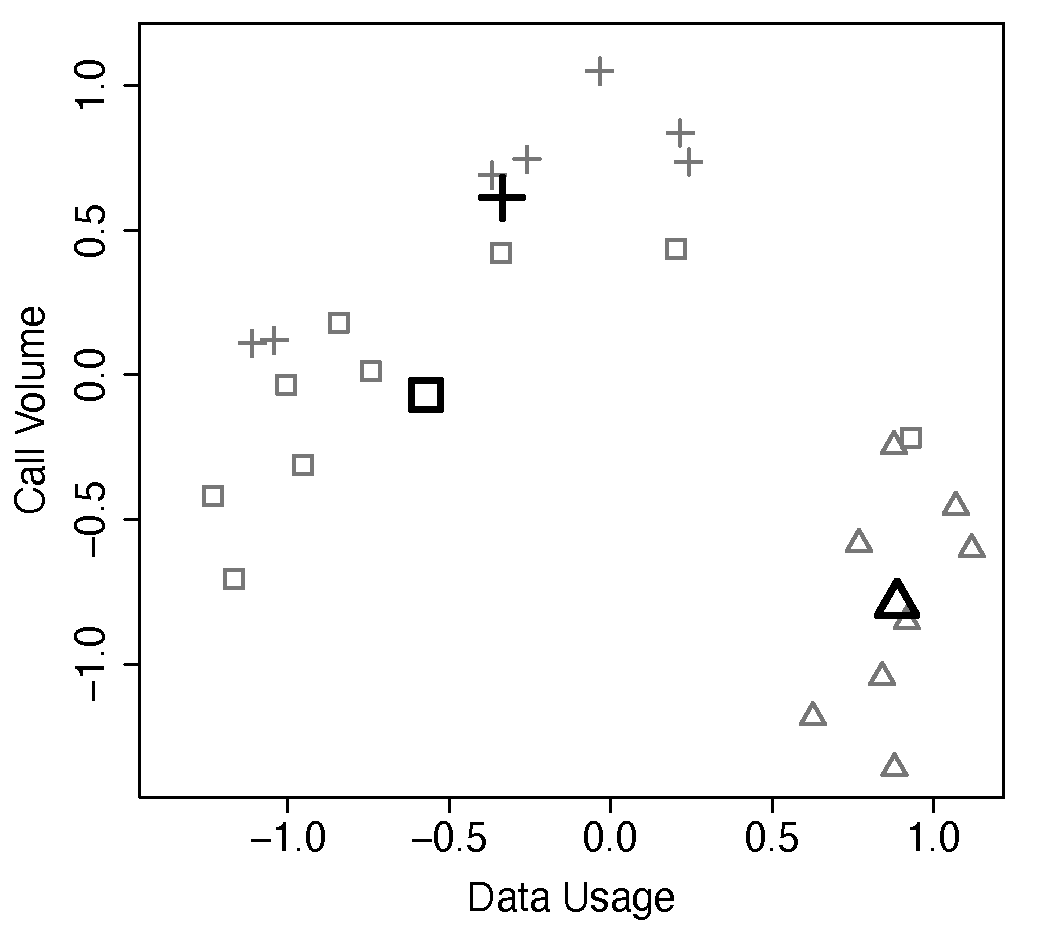
\includegraphics[width=0.22\linewidth]{./images/fmlpda_figure_10_3_d.pdf}} &
	\subfigure[]{\label{fig:kmeansDemo5}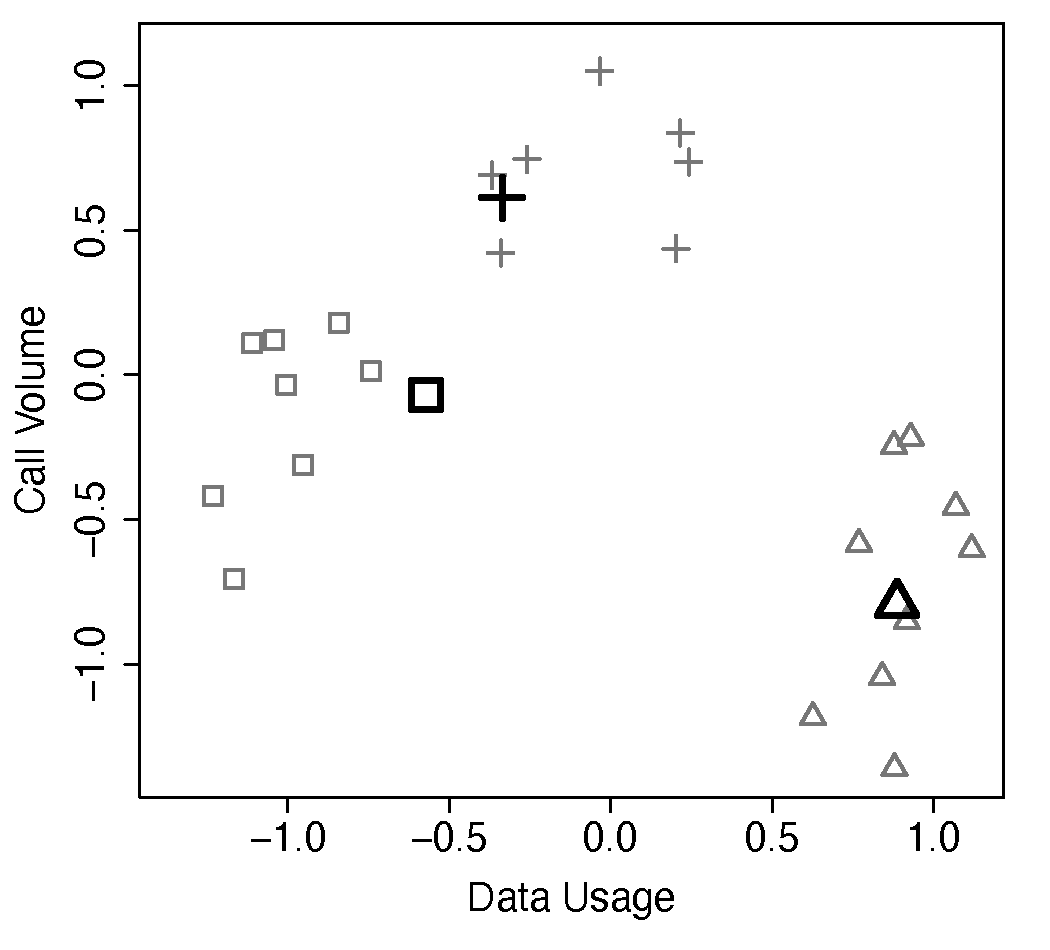
\includegraphics[width=0.22\linewidth]{./images/fmlpda_figure_10_3_e.pdf}} &
	\subfigure[]{\label{fig:kmeansDemo6}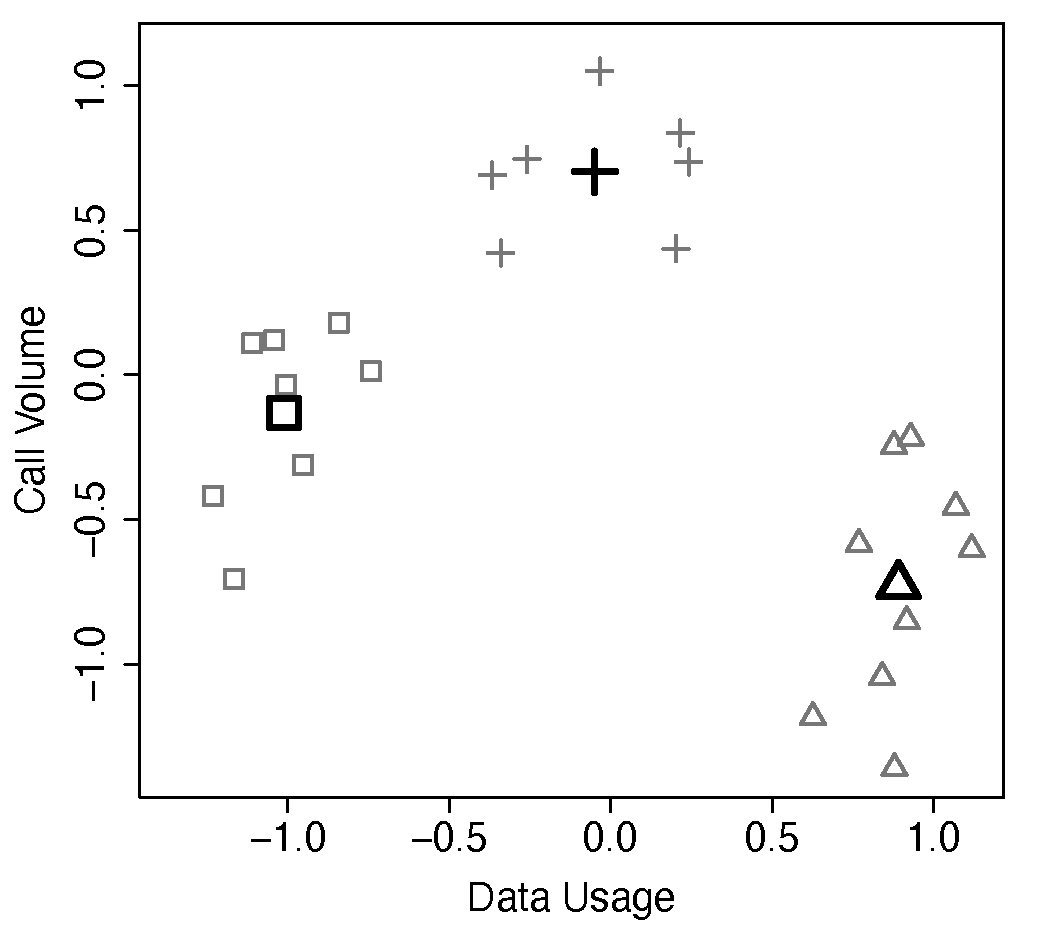
\includegraphics[width=0.22\linewidth]{./images/fmlpda_figure_10_3_f.pdf}} \\
	
\end{tabular}
}	
\caption{(a) A plot of the mobile phone customer dataset given in Table \ourRef{table:kmeansDemoData}. (b)--(f) The progress of the \textit{k}-means clustering algorithm, working on the simple customer segmentation dataset. The large symbols represent cluster centroids, and the smaller symbols represent cluster assignments.}
\label{fig:kmeansDemoDataProcess}
\end{figure}
\end{frame} 



 \begin{frame} 
 \begin{scriptsize}
\begin{eqnarray*}
{\mathbf{c}_1}[\featN{Data Usage}] & = & (-0.9531 + -1.167 + -1.2329 + -0.8431 + 0.9285 \\
~ & ~ & ~~~~~~~~~ + -1.005 + 0.2021 + -0.7426 + -0.3414 )/9 \\
~ & = & -0.5727 \\
{\mathbf{c}_1}[\featN{Call Volume}] & = & (-0.3107 + -0.706 + -0.4188 + 0.1811  + -0.2168  \\
~ & ~ & ~~~~~~~~~ + -0.0337  + 0.4364  + 0.0119  + 0.4215 )/9 \\
~ & = & -0.0706 \\
\end{eqnarray*}
 \end{scriptsize}
\end{frame} 



 \begin{frame} 
\begin{eqnarray*}
\mathcal{C}_1 & = & \left\{\mathbf{d}_{1}, \mathbf{d}_{2}, \mathbf{d}_{3}, \mathbf{d}_{5}, \mathbf{d}_{6}, \mathbf{d}_{11}, \mathbf{d}_{19}, \mathbf{d}_{20}\right\} \\ 
\mathcal{C}_2 & = & \left\{\mathbf{d}_{4}, \mathbf{d}_{8}, \mathbf{d}_{9}, \mathbf{d}_{10}, \mathbf{d}_{15}, \mathbf{d}_{17}, \mathbf{d}_{18}, \mathbf{d}_{21}, \mathbf{d}_{22}\right\} \\ 
\mathcal{C}_3 & = & \left\{\mathbf{d}_{7}, \mathbf{d}_{12}, \mathbf{d}_{13}, \mathbf{d}_{14}, \mathbf{d}_{16}, \mathbf{d}_{23}, \mathbf{d}_{24}\right\} \\ 
\end{eqnarray*}
\end{frame} 


\SectionSlide{Extensions and Variations}


\subsection{Choosing Initial Cluster Centroids}



 \begin{frame} 
\begin{figure}[!htb]
{\setlength{\tabcolsep}{0.05em}
\begin{tabular}{cccc}
	\subfigure[Seed]{\label{fig:kmeansDifferentSeeds1a}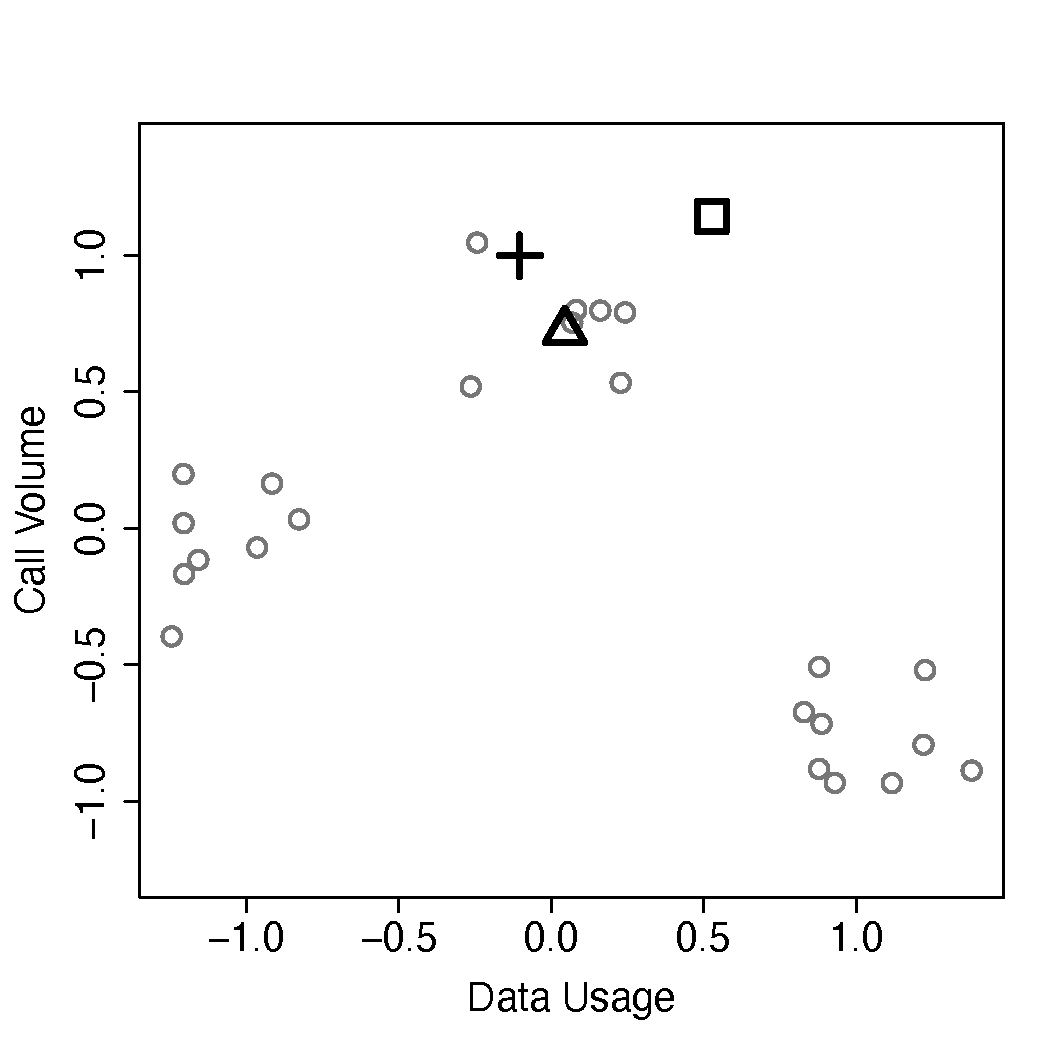
\includegraphics[width=0.245\linewidth]{./images/fmlpda_figure_10_4_a.pdf}}&
	\subfigure[Clustering]{\label{fig:kmeansDifferentSeeds1b}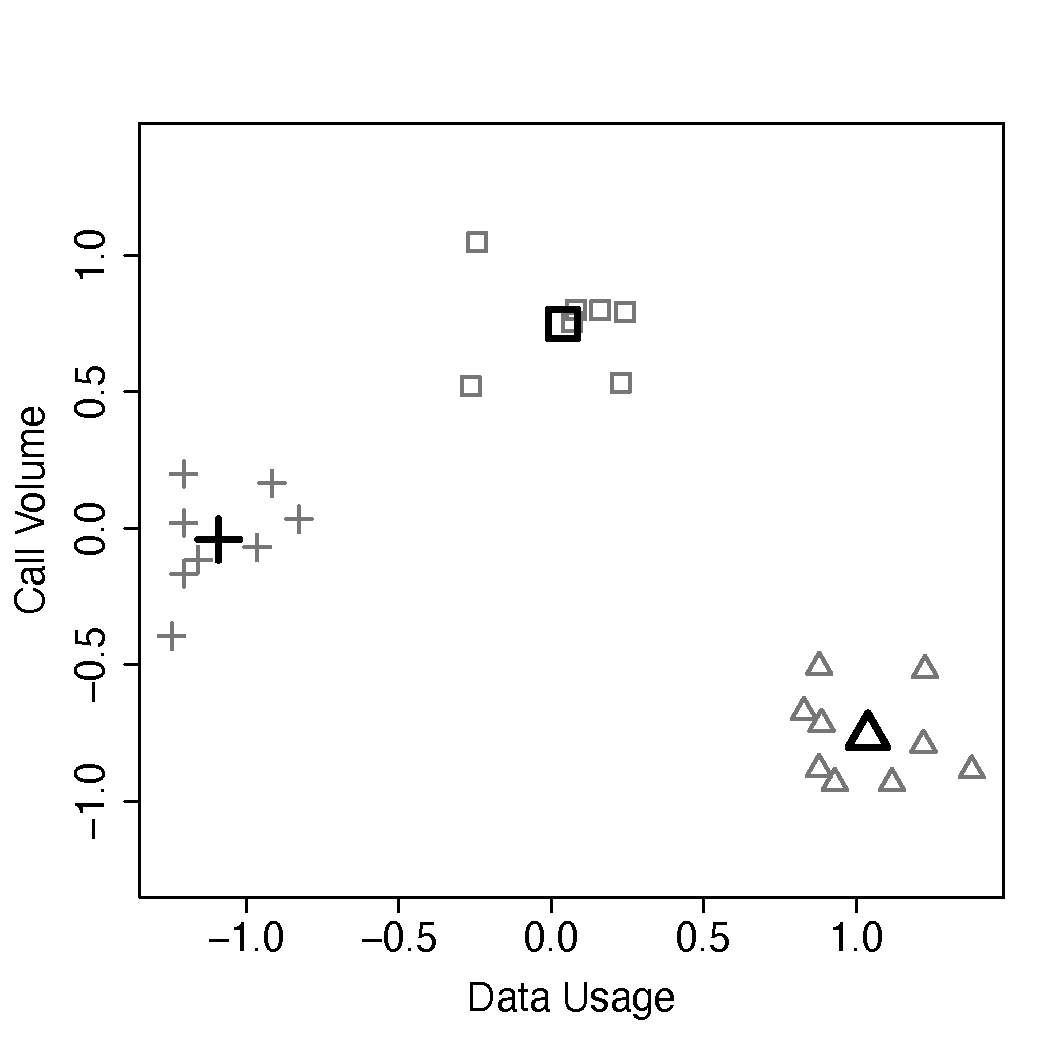
\includegraphics[width=0.245\linewidth]{./images/fmlpda_figure_10_4_b.pdf}} & 
	\subfigure[Seed]{\label{fig:kmeansDifferentSeeds2a}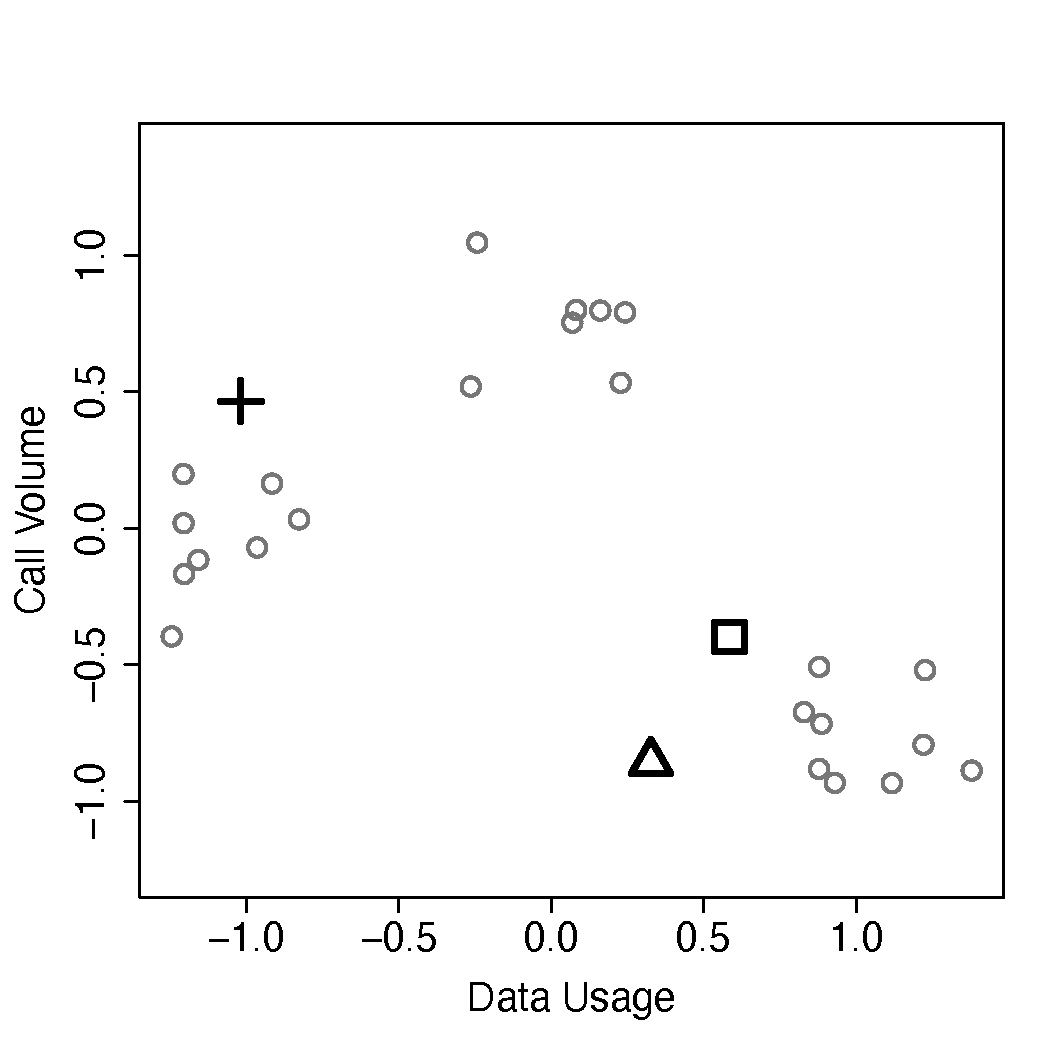
\includegraphics[width=0.245\linewidth]{./images/fmlpda_figure_10_4_c.pdf}} &
	\subfigure[Clustering]{\label{fig:kmeansDifferentSeeds2b}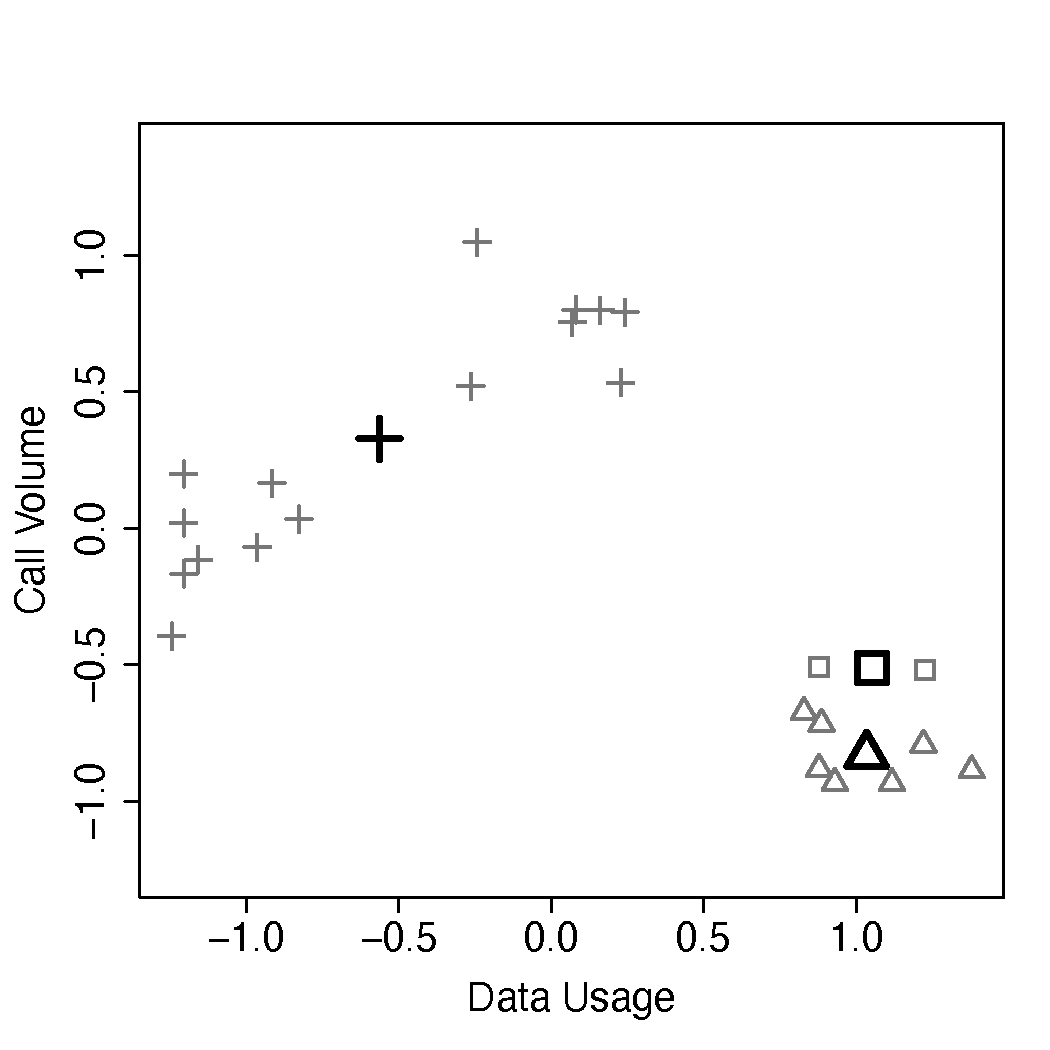
\includegraphics[width=0.245\linewidth]{./images/fmlpda_figure_10_4_d.pdf}} \\
	
	\subfigure[Seed]{\label{fig:kmeansDifferentSeeds3a}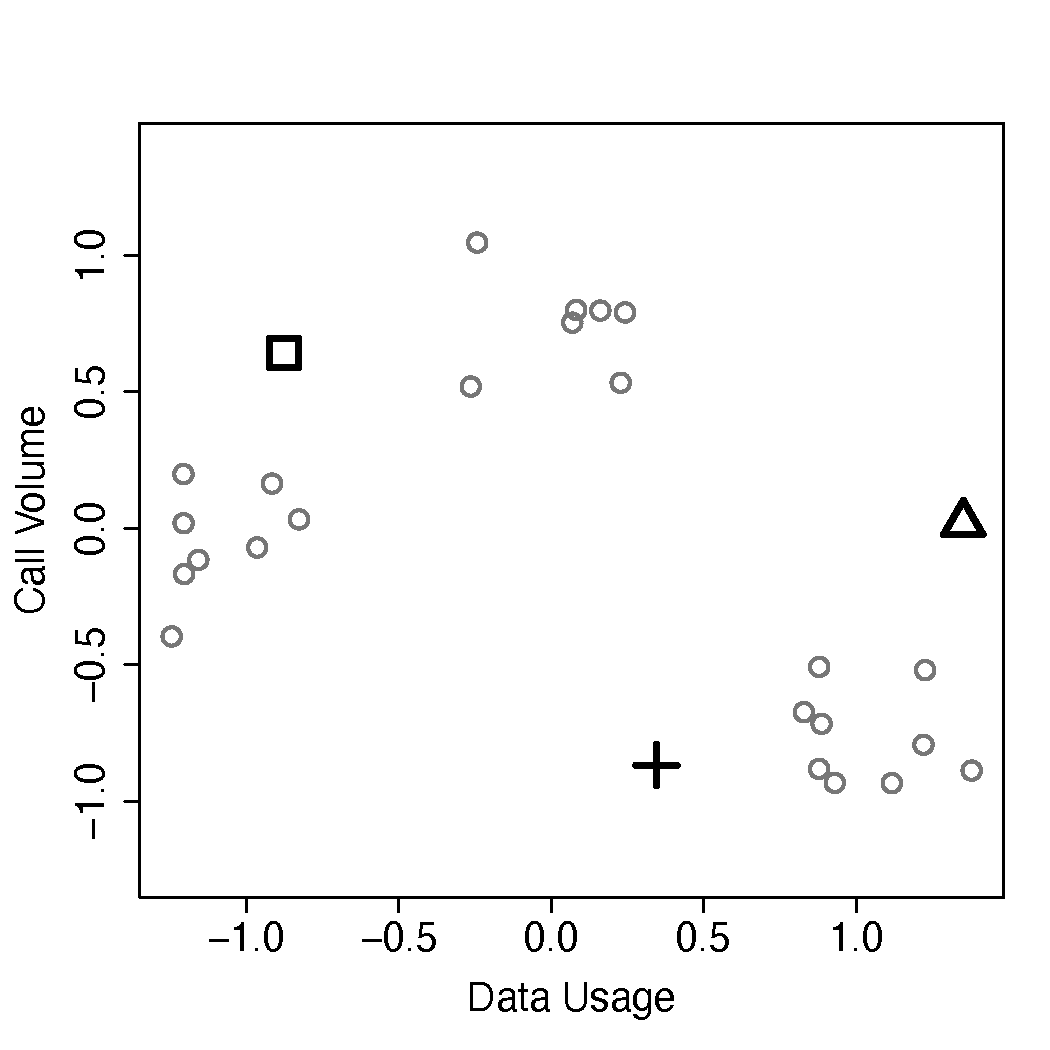
\includegraphics[width=0.245\linewidth]{./images/fmlpda_figure_10_4_e.pdf}}&
	\subfigure[Clustering]{\label{fig:kmeansDifferentSeeds3b}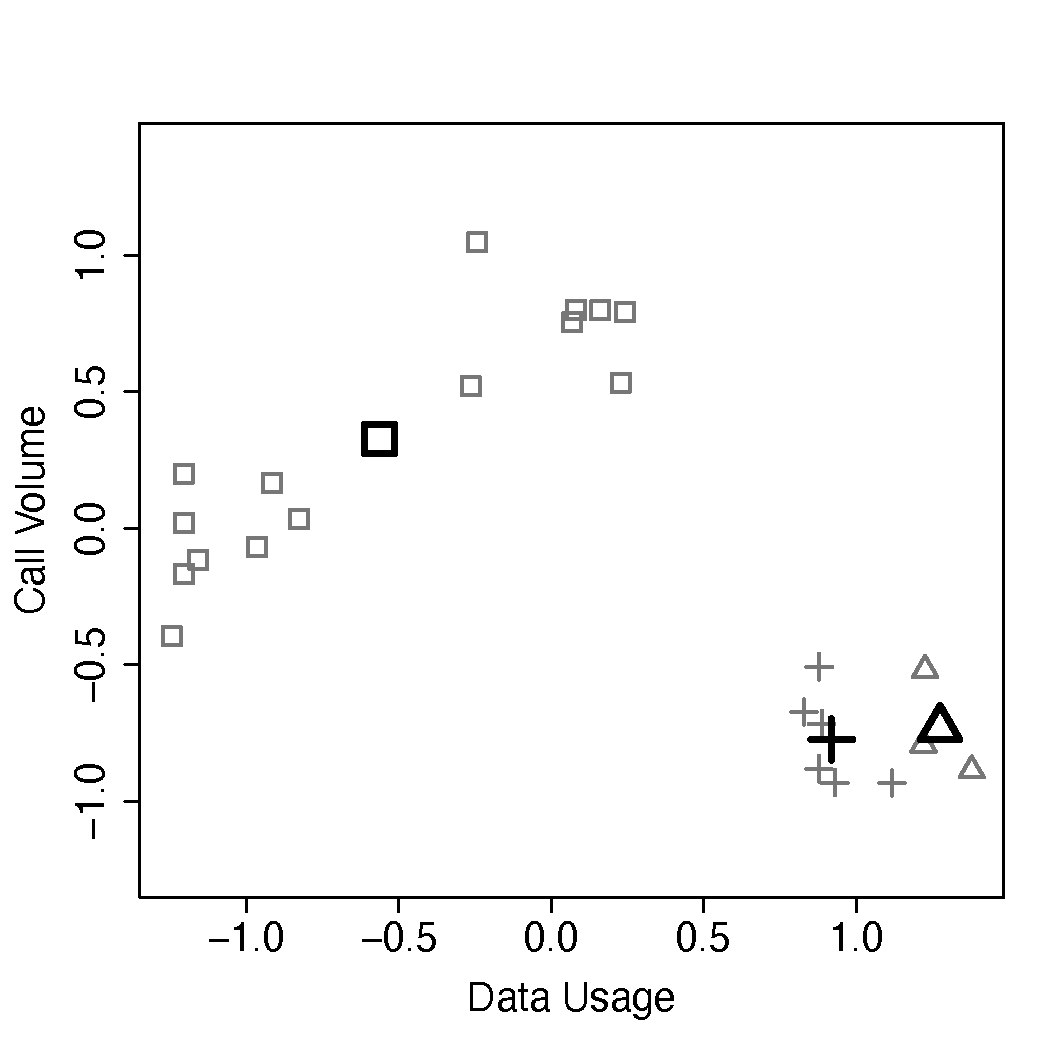
\includegraphics[width=0.245\linewidth]{./images/fmlpda_figure_10_4_f.pdf}} & 
	\subfigure[Seed]{\label{fig:kmeansDifferentSeeds4a}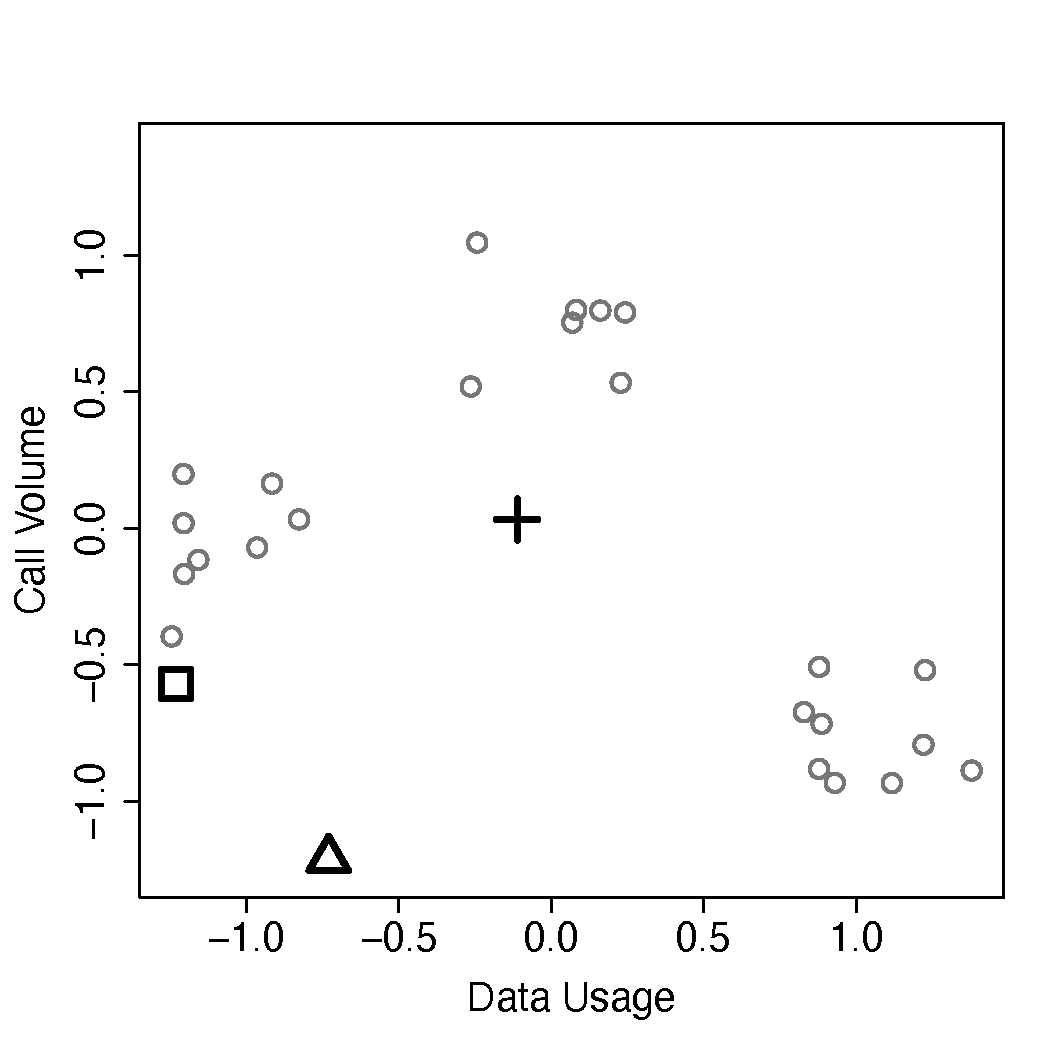
\includegraphics[width=0.245\linewidth]{./images/fmlpda_figure_10_4_g.pdf}} &
	\subfigure[Clustering]{\label{fig:kmeansDifferentSeeds4b}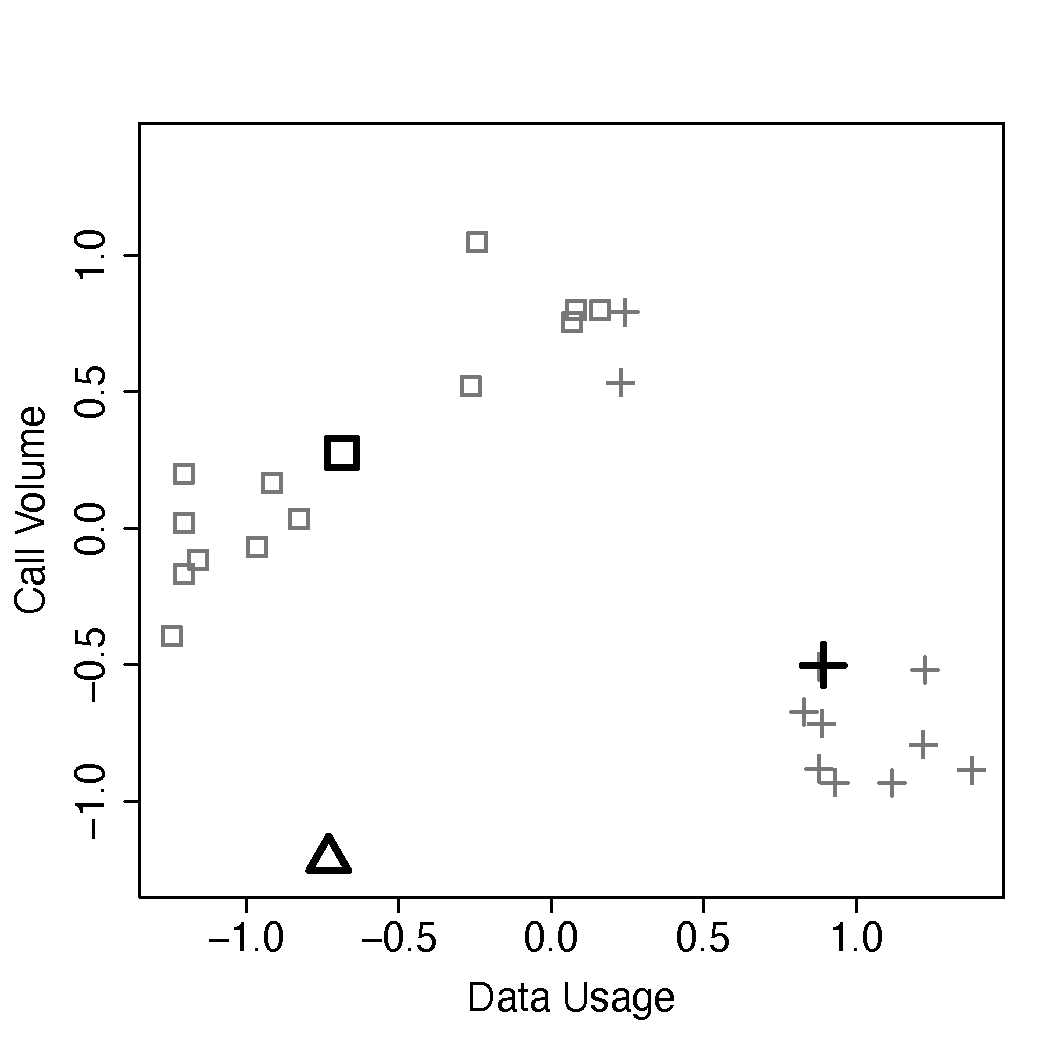
\includegraphics[width=0.245\linewidth]{./images/fmlpda_figure_10_4_h.pdf}} \\
	
\end{tabular}
}	
\caption{(a)--(h) Different clusterings (all with $k=3$) that can be found for the mobile phone customer dataset given in Table \ourRef{table:kmeansDemoData} when different initial cluster centroids are used.}
\label{fig:kmeansDifferentSeeds}
\end{figure}
\end{frame} 


\begin{frame}[plain]
\scriptsize{Pseudocode description of the \keyword{k-means++} algorithm.}
\begin{footnotesize}
%\begin{algorithm}[htb]
%\caption{Pseudocode description of the \keyword{k-means++} algorithm.}
%\label{alg:kemeans++}
\begin{algorithmic}[1]
\Require a dataset $\mathcal{D}$ containing $n$ training instances, $\mathbf{d}_1, \ldots, \mathbf{d}_n$ 
\Require $k$, the number of cluster centroids to find 
\Require a distance measure ${Dist}$ to compare instances to cluster centroids
\State choose $\mathbf{d}_i$ randomly (following a uniform distribution) from $\mathcal{D}$ to be the position of the initial centroid, ${\mathbf{c}_1}$, of the first cluster, $\mathcal{C}_1$   
\For{cluster $\mathcal{C}_j$ in $\mathcal{C}_2$ to $\mathcal{C}_k$}
    \State{for each instance, $\mathbf{d}_i$, in $\mathcal{D}$ let ${Dist}(\mathbf{d}_i)$ be the distance between $\mathbf{d}_i$ and its nearest cluster centroid}
    \State{calculate a selection weight for each instance, $\mathbf{d}_i$, in $\mathcal{D}$ as $\displaystyle{\frac{{Dist}(\mathbf{d}_i)^2}{\sum_{p=1}^n{{Dist}(\mathbf{d}_p)^2}}}$ }
    \State{choose $\mathbf{d}_i$ as the position of cluster centroid, ${\mathbf{c}_j}$, for cluster $\mathcal{C}_j$ randomly following a distribution based on the selection weights}
\EndFor
\State proceed with \textit{k}-means as normal using $\left\{{\mathbf{c}_1}, \ldots, {\mathbf{c}_k}\right\}$ as the initial centroids.
\end{algorithmic}
%\end{algorithm}
\end{footnotesize}
\end{frame}



 \begin{frame} 
\begin{figure}[!htb]
{\setlength{\tabcolsep}{0.05em}
\begin{tabular}{cccc}
	\subfigure[]{\label{fig:kmeans++Seeds1}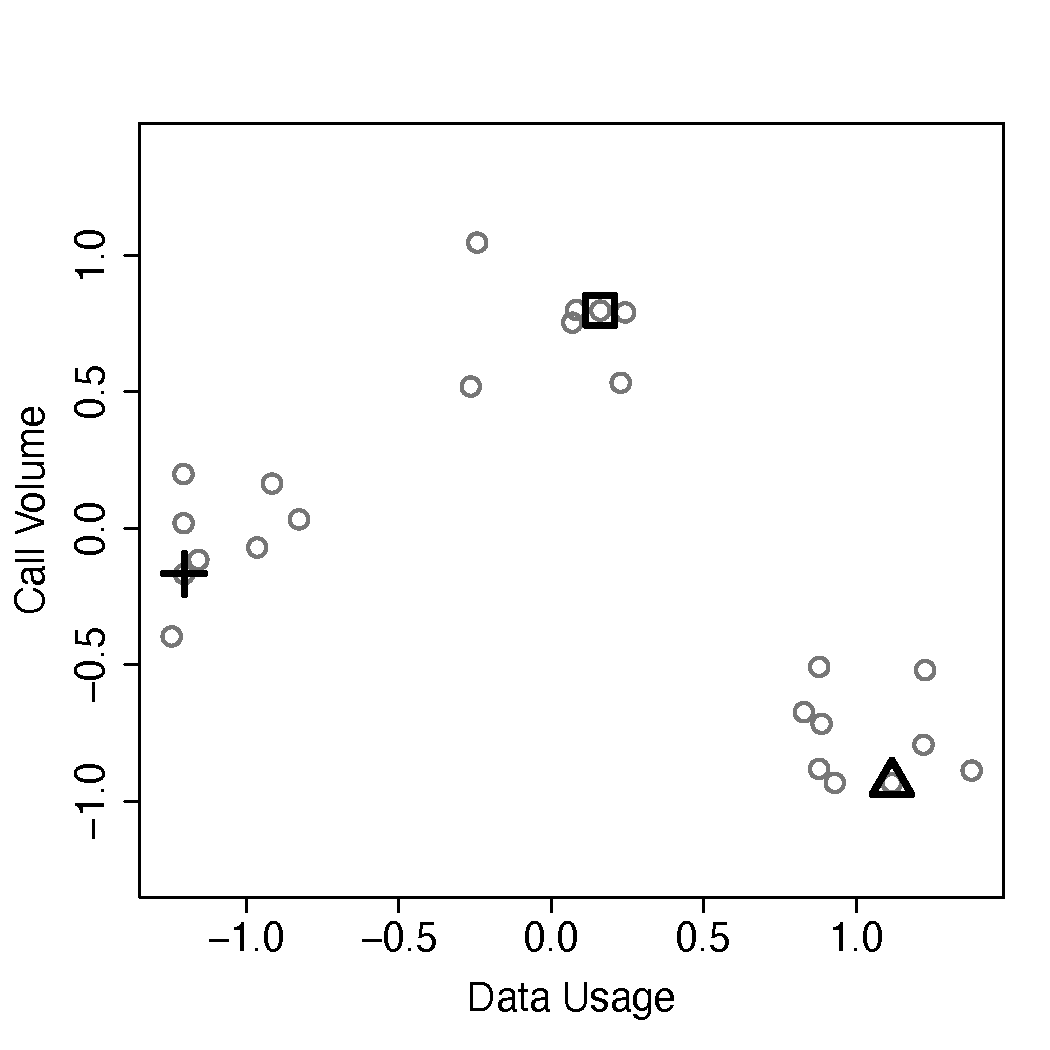
\includegraphics[width=0.245\linewidth]{./images/fmlpda_figure_10_5_a.pdf}}&
	\subfigure[]{\label{fig:kmeans++Seeds2}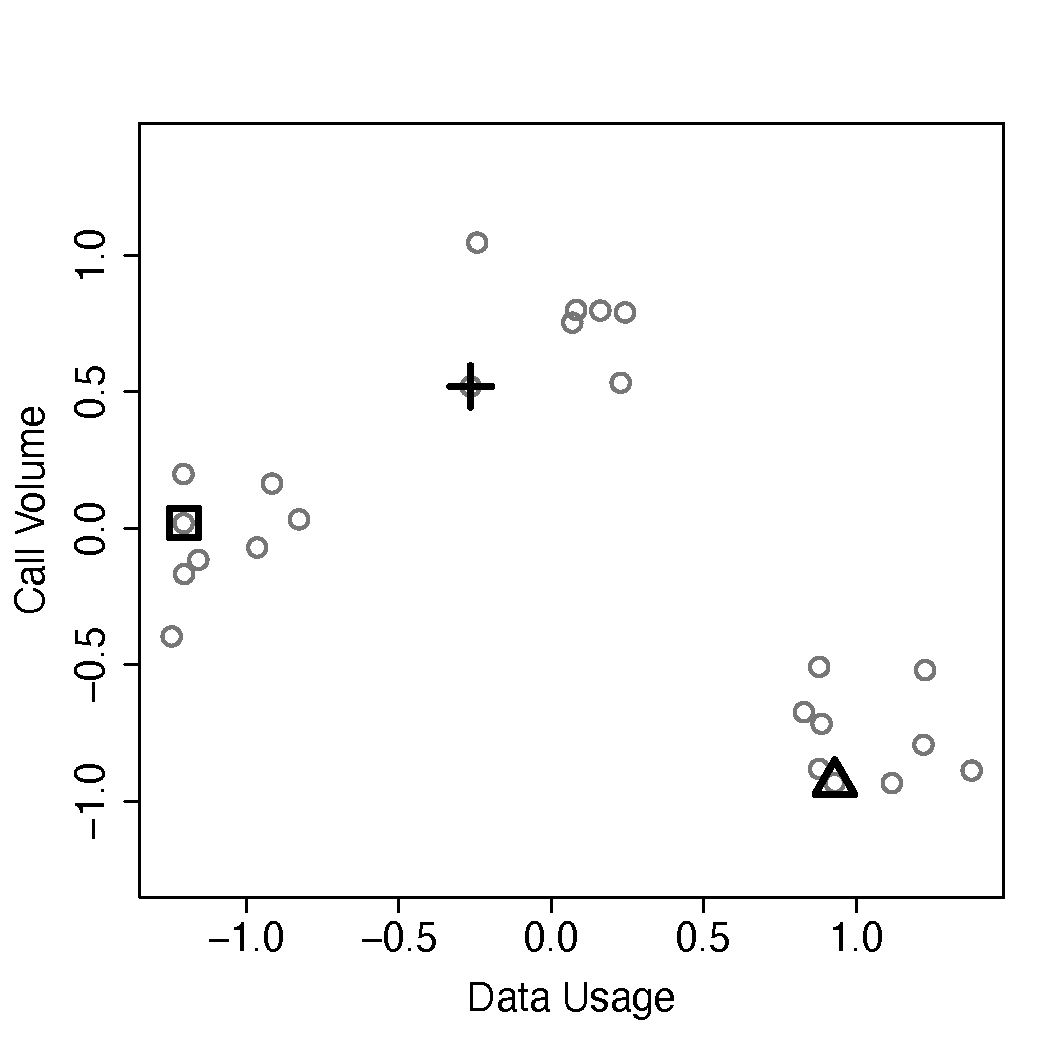
\includegraphics[width=0.245\linewidth]{./images/fmlpda_figure_10_5_b.pdf}} & 
	\subfigure[]{\label{fig:kmeans++Seeds3}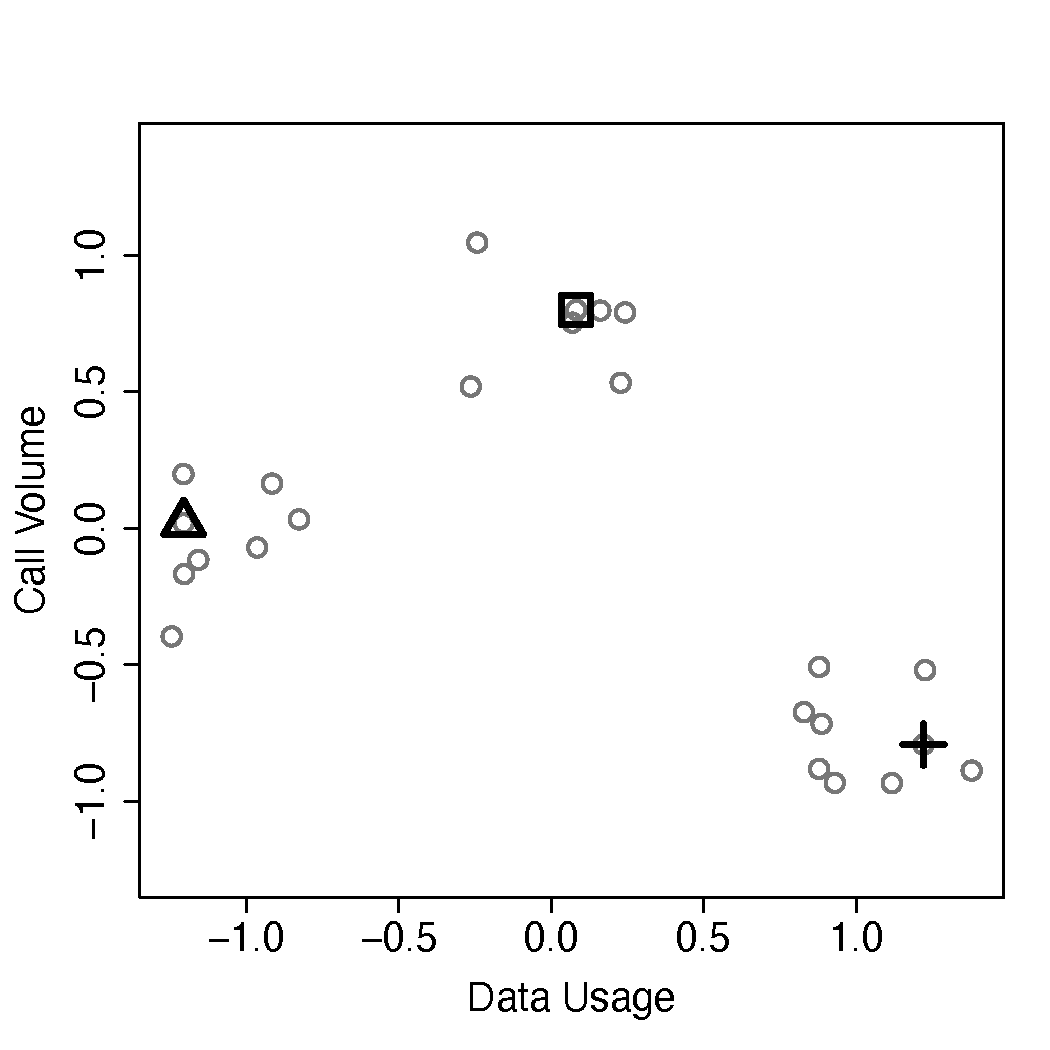
\includegraphics[width=0.245\linewidth]{./images/fmlpda_figure_10_5_c.pdf}} &
	\subfigure[]{\label{fig:kmeans++Seeds4}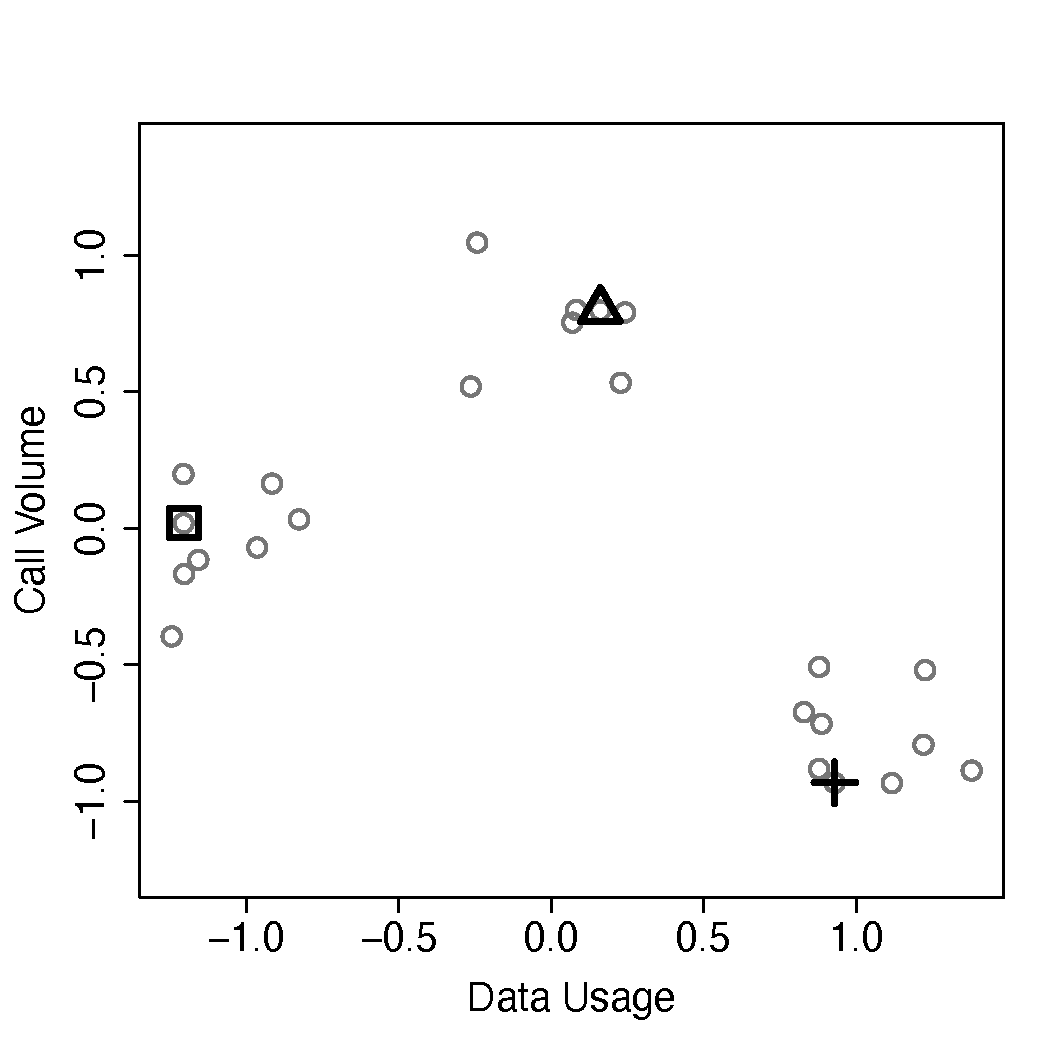
\includegraphics[width=0.245\linewidth]{./images/fmlpda_figure_10_5_d.pdf}} \\
\end{tabular}
}	
\caption{(a)--(d) Initial centroids chosen using the k-means++ approach (all with $k=3$) for the mobile phone customer dataset given in Table \ourRef{table:kmeansDemoData}.}
\label{fig:kmeans++Seeds}
\end{figure}
\end{frame} 


\subsection{Evaluating Clustering}



 \begin{frame} 
\begin{figure}[!htb]
{\setlength{\tabcolsep}{0.05em}
\begin{center}
\begin{scriptsize}
\begin{tabular}{cccc}
	\subfigure[]{\label{fig:clustDistIntra}\includegraphics[width=0.26\textwidth]{./images/fmlpda_figure_10_6_a.pdf}}&
	\subfigure[]{\label{fig:clustDistInter}\includegraphics[width=0.26\textwidth]{./images/fmlpda_figure_10_6_b.pdf}}  &
	\subfigure[]{\label{fig:clustDistExGood}\includegraphics[width=0.26\textwidth]{./images/fmlpda_figure_10_6_c.pdf}} &
	\subfigure[]{\label{fig:clustDistExBad}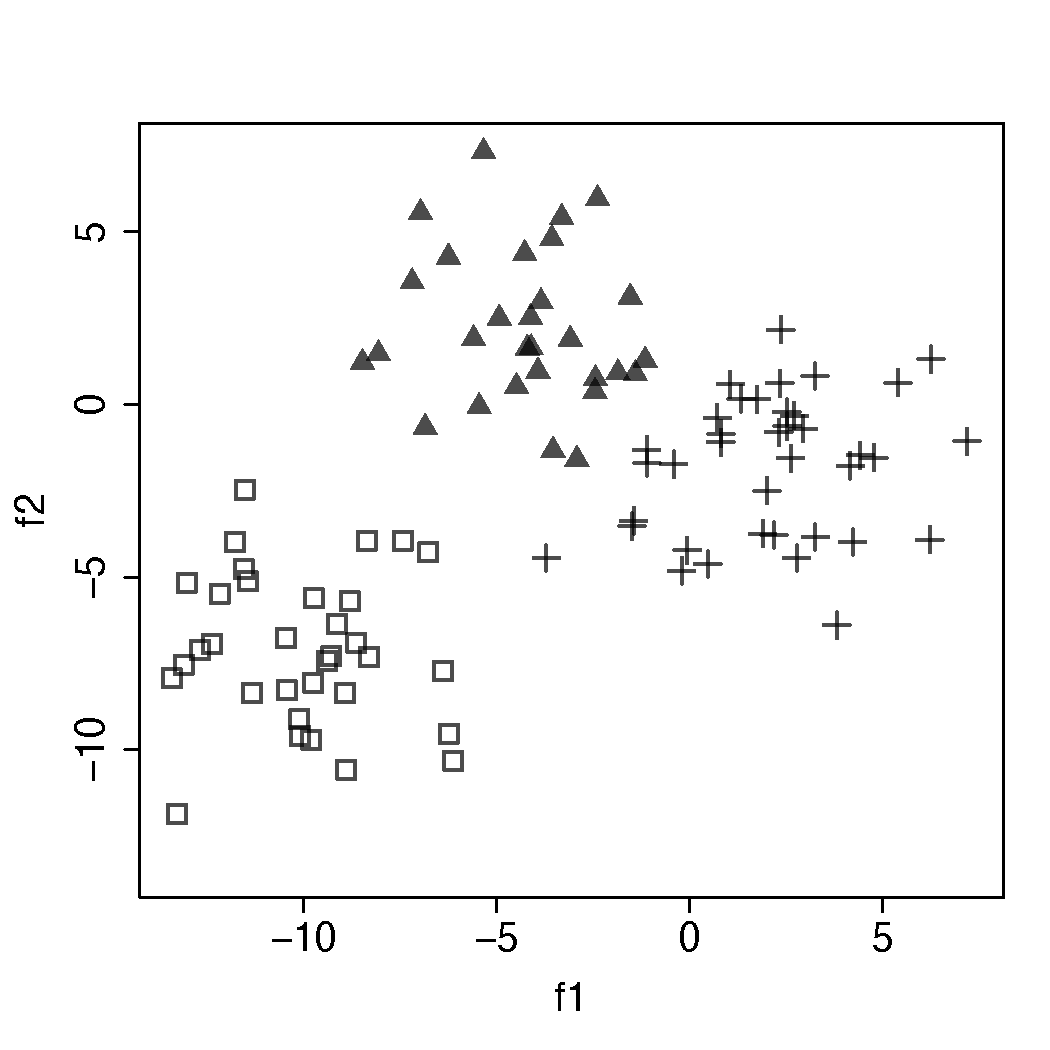
\includegraphics[width=0.26\textwidth]{./images/fmlpda_figure_10_6_d.pdf}} \\
	
\end{tabular}
\end{scriptsize}
\end{center}
}	
\caption{(a) Intra-cluster distance; (b) inter-cluster distance; (c) a \textit{good} clustering; and (d) a \textit{bad} clustering.}
\label{fig:clustDists}
\end{figure}
\end{frame} 



 \begin{frame} 
    \begin{equation}
    s(i)= \frac{b(i)-a(i)}{\max(a(i), b(i))}
    \label{eqn:silhouette_width}
    \end{equation}
\end{frame} 


\begin{frame}

\noindent \includegraphics[width=0.8\textwidth]{images/fmlpda_eqn_10_1.pdf}

\noindent \includegraphics[width=\textwidth]{images/fmlpda_eqn_10_2.pdf}

\noindent \includegraphics[width=0.8\textwidth]{images/fmlpda_eqn_10_3.pdf}

\end{frame}


% \begin{frame} 
%\begin{equation*}
%\label{eqn:silhouette_example_dist_matrix_1}
%\begin{footnotesize}
%    \kbordermatrix{ & \mathbf{d}_{2} &\mathbf{d}_{3} &\mathbf{d}_{5} &\mathbf{d}_{6} &\mathbf{d}_{11} &\mathbf{d}_{19} &\mathbf{d}_{20}  \\
%\mathbf{d}_{1} & 0.45 & 0.30 & 0.45 & 0.50 & 0.28 & 0.44 & 0.39 }\\ 
%\end{footnotesize}
%\end{equation*}
%\end{frame} 
%
%
%
% \begin{frame} 
%\begin{equation*}
%\label{eqn:silhouette_example_dist_matrix_2}
%\begin{footnotesize}
%    \kbordermatrix{ & \mathbf{d}_{4} &\mathbf{d}_{8} &\mathbf{d}_{9} &\mathbf{d}_{10} &\mathbf{d}_{15} &\mathbf{d}_{17} &\mathbf{d}_{18} &\mathbf{d}_{21} &\mathbf{d}_{22} \\
%\mathbf{d}_{1} & 2.03 & 1.88 & 2.09 & 1.94 & 1.83 & 2.11 & 1.95 & 1.80 & 1.74} \\
%\end{footnotesize}
%\end{equation*}
%\end{frame} 
%
%
%
% \begin{frame} 
%\begin{equation*}
%\label{eqn:silhouette_example_dist_matrix_3}
%\begin{footnotesize}
%    \kbordermatrix{ & \mathbf{d}_{7} &\mathbf{d}_{12} &\mathbf{d}_{13} &\mathbf{d}_{14} &\mathbf{d}_{16} &\mathbf{d}_{23} &\mathbf{d}_{24}  \\
%\mathbf{d}_{1} & 1.16 & 1.59 & 1.38 & 1.64 & 1.64 & 1.26 & 0.95 }\\ 
%\end{footnotesize}
%\end{equation*}
%\end{frame} 



 \begin{frame} 
\begin{equation*}
\frac{1.3743 - 0.401}{max(0.401, 1.374)} = 0.7081
\end{equation*}
\end{frame} 



\begin{frame}[plain]
\scriptsize{Pseudocode description of the algorithm for calculating the \keyword{silhouette} for internal cluster evaluation.}
\begin{footnotesize}
%\begin{algorithm}[htb]
%\caption{Pseudocode description of the algorithm for calculating the \keyword{silhouette} for internal cluster evaluation.}
%\label{alg:silhouette}
\begin{algorithmic}[1]
\Require a dataset $\mathcal{D}$ containing $n$ training instances, $\mathbf{d}_1, \ldots, \mathbf{d}_n$ 
\Require a clustering $\mathbf{\mathcal{C}}$ of dataset $\mathcal{D}$ into $k$ clusters, $\mathcal{C}_{1}, \ldots, \mathcal{C}_{k}$ 
\Require a distance measure, ${Dist}$, to compare distances between instances
    \For{each instance $\mathbf{d}_i$ in $\mathcal{D}$}
    \State{let $a(i)$ be the average distance between instance $\mathbf{d}_i$ and all of the other instances within the cluster to which $\mathbf{d}_i$ belongs, $\mathcal{C}_{j}$ (\textit{average intra-cluster distance})}
    \State{calculate the average distance between instance $\mathbf{d}_i$ and the members of each of the other clusters $\mathcal{C}~\setminus~\mathcal{C}_{j}$}
    \State{let $b(i)$ be the lowest average distance between instance $\mathbf{d}_i$ and any other cluster (\textit{average inter-cluster distance})}
    \State  calculate the silhouette index for $\mathbf{d}_i$ as
%    \begin{equation}
%    s(i)= 
%    \begin{cases}
%        1-a(i)/b(i) & \text{if } a(i) \le b(i)\\
%        0 & \text{if } a(i) = b(i)\\
%        b(i)/a(i)-1 & \text{if } a(i) \ge b(i)\\
%    \end{cases}
%    \end{equation}
    \begin{equation}
    s(i)= \frac{b(i)-a(i)}{\max(a(i), b(i))}
    \label{eqn:silhouette_width}
    \end{equation}
\EndFor
\State calculate final silhouette for the clustering as  $ \displaystyle s = \frac{1}{n}\sum_{i=1}^n{s(i)}$ 
\end{algorithmic}
%\end{algorithm}
\end{footnotesize}
\end{frame}






 \begin{frame} 
\begin{table}[!t]
\caption{Calculating the silhouette for the final clustering of the mobile phone customer dataset (Table \ourRef{table:kmeansDemoData}) found using the \textit{k}-means algorithm (with $k=3$). The overall silhouette index value is $0.66$. }
\label{table:silhouetteDemo}
\begin{scriptsize}
{\setlength{\tabcolsep}{0em}
\begin{tabular}{cc}
\Toprule
\begin{minipage}{0.5\textwidth}
\raggedright
{\setlength{\tabcolsep}{0.1em}
	\begin{tabular*}{12.0pc}{@{\extracolsep{\fill}} rrrrrr @{}}
~	 & ~ & Nearest &  ~ \\
\featN{ID}	 & Cluster & Cluster & $a(i)$ & $b(i)$ & $s(i)$ \\
\Midrule
1 & $\mathcal{C}_1$ & $\mathcal{C}_3$ & 0.401 & 1.374 & 0.708 \\ 
2 & $\mathcal{C}_1$ & $\mathcal{C}_3$ & 0.695 & 1.811 & 0.616 \\ 
3 & $\mathcal{C}_1$ & $\mathcal{C}_3$ & 0.503 & 1.644 & 0.694 \\ 
4 & $\mathcal{C}_2$ & $\mathcal{C}_3$ & 0.484 & 1.628 & 0.703 \\ 
5 & $\mathcal{C}_1$ & $\mathcal{C}_3$ & 0.387 & 1.232 & 0.686 \\ 
6 & $\mathcal{C}_1$ & $\mathcal{C}_3$ & 0.445 & 0.970 & 0.541 \\ 
7 & $\mathcal{C}_3$ & $\mathcal{C}_1$ & 0.452 & 1.056 & 0.572 \\ 
8 & $\mathcal{C}_2$ & $\mathcal{C}_3$ & 0.599 & 1.364 & 0.561 \\ 
9 & $\mathcal{C}_2$ & $\mathcal{C}_3$ & 0.470 & 1.768 & 0.734 \\ 
10 & $\mathcal{C}_2$ & $\mathcal{C}_3$ & 0.504 & 1.978 & 0.745 \\ 
11 & $\mathcal{C}_1$ & $\mathcal{C}_3$ & 0.327 & 1.223 & 0.732 \\ 
12 & $\mathcal{C}_3$ & $\mathcal{C}_1$ & 0.433 & 1.537 & 0.719 \\ 
\Botrule
\end{tabular*}
}
\end{minipage}
&
\begin{minipage}{0.5\textwidth}
\raggedleft
{\setlength{\tabcolsep}{0.1em}
	\begin{tabular*}{12.0pc}{@{\extracolsep{\fill}} rrrrrr @{}}
~	 & ~ & Nearest &  ~ \\
\featN{ID}	 & Cluster & Cluster & $a(i)$ & $b(i)$ & $s(i)$ \\
\Midrule
13 & $\mathcal{C}_3$ & $\mathcal{C}_1$ & 0.5136 & 1.3592 & 0.6221 \\ 
14 & $\mathcal{C}_3$ & $\mathcal{C}_1$ & 0.4349 & 1.5738 & 0.7236 \\ 
15 & $\mathcal{C}_2$ & $\mathcal{C}_3$ & 0.5776 & 1.3480 & 0.5715 \\ 
16 & $\mathcal{C}_3$ & $\mathcal{C}_1$ & 0.4955 & 1.5409 & 0.6784 \\ 
17 & $\mathcal{C}_2$ & $\mathcal{C}_1$ & 0.7369 & 2.2757 & 0.6762 \\ 
18 & $\mathcal{C}_2$ & $\mathcal{C}_3$ & 0.4312 & 1.8473 & 0.7666 \\ 
19 & $\mathcal{C}_1$ & $\mathcal{C}_3$ & 0.3711 & 1.1682 & 0.6823 \\ 
20 & $\mathcal{C}_1$ & $\mathcal{C}_3$ & 0.4334 & 1.0006 & 0.5669 \\ 
21 & $\mathcal{C}_2$ & $\mathcal{C}_1$ & 0.6520 & 1.9710 & 0.6692 \\ 
22 & $\mathcal{C}_2$ & $\mathcal{C}_3$ & 0.4504 & 1.5457 & 0.7086 \\ 
23 & $\mathcal{C}_3$ & $\mathcal{C}_1$ & 0.3954 & 1.1654 & 0.6607 \\ 
24 & $\mathcal{C}_3$ & $\mathcal{C}_1$ & 0.5339 & 0.8880 & 0.3988 \\ 
\Botrule
\end{tabular*}
}
\end{minipage}\\
\end{tabular}
}
{}
\end{scriptsize}
\end{table}
\end{frame} 



 \begin{frame} 
\begin{figure}[tbh]
       \begin{centering}
			\includegraphics[width=0.8\textwidth]{images/fmlpda_figure_10_7.pdf}
       \caption{The silhouette plot for the final clustering of the mobile phone customer dataset (Table \ourRef{table:kmeansDemoData}) found using the \textit{k}-means algorithm (with $k=3$).}
       \label{fig:demoSilhouette}
       \end{centering}
\end{figure}
\end{frame} 


\subsection{Choosing the Number of Clusters}



 \begin{frame} 
\begin{figure}[!t]
{\setlength{\tabcolsep}{0.05em}
\begin{center}
\begin{tabular}{cccc}

	\subfigure[$k = 2$]{\label{fig:silhouetteKDemo2}\includegraphics[width=0.245\linewidth]{./images/fmlpda_figure_10_8_a.pdf}}&
	\subfigure[$k = 3$]{\label{fig:silhouetteKDemo3}\includegraphics[width=0.245\linewidth]{./images/fmlpda_figure_10_8_b.pdf}} &
	\subfigure[$k = 4$]{\label{fig:silhouetteKDemo4}\includegraphics[width=0.245\linewidth]{./images/fmlpda_figure_10_8_c.pdf}}&
	\subfigure[$k = 5$]{\label{fig:silhouetteKDemo5}\includegraphics[width=0.245\linewidth]{./images/fmlpda_figure_10_8_d.pdf}} \\
	
	\subfigure[$k = 6$]{\label{fig:silhouetteKDemo6}\includegraphics[width=0.245\linewidth]{./images/fmlpda_figure_10_8_e.pdf}}&
	\subfigure[$k = 7$]{\label{fig:silhouetteKDemo7}\includegraphics[width=0.245\linewidth]{./images/fmlpda_figure_10_8_f.pdf}} &
	\multicolumn{2}{l}{\subfigure[Silhouette summary]{\label{fig:silhouetteKDemoOverview}\includegraphics[width=0.32\linewidth]{./images/fmlpda_figure_10_8_g.pdf}}}  \\	
\end{tabular}
\end{center}
}	
\caption{(a)--(f) Different clusterings found for the mobile phone customer dataset in Table \ourRef{table:kmeansDemoData} for values of $k$ in $(2, 9)$. (g) shows the silhouette for each clustering.}
\label{fig:silhouetteKDemo}
\end{figure}
\end{frame} 


\subsection{Understanding Clustering Results}



 \begin{frame} 
\begin{table}[!t]
\caption{Summary statistics for the three clusters found in the mobile phone customer dataset in Table \ourRef{table:kmeansDemoData} using \textit{k}-means clustering ($k=3$). Note, that the \% missing and cardinality columns usually used are omitted here for legibility as these data quality issues will not arise in this simple example. They could be included when this approach is used on \textit{real} datasets.}
\label{table:explainingClustering_C1}
\begin{scriptsize}
{\setlength{\tabcolsep}{0.3em}
\begin{tabular*}{\textwidth}{@{\extracolsep{\fill}} p{1.3cm} l rrrrrrrrr @{}}
\Toprule
~ & ~ & ~ & ~ & $1^{st}$ & ~ & ~ & $3^{rd}$ & ~ & Std. \\ 
Feature & Cluster & Count & Min. & Qrt. & Mean & Median & Qrt. & Max & Dev. \\ 
\Midrule
\multirow{3}{1.3cm}{\featN{Data} \featN{Usage}} &  $\mathcal{C}_1$ & 8 & -1.2329 & -1.1246 & -1.0121 & -1.0237 & -0.9256 & -0.7426 & 0.1639\\ 
~ & $\mathcal{C}_2$ & 9 & 0.6259 & 0.8404 & 0.8912 & 0.8785 & 0.9285 & 1.1175 & 0.1471 \\ 
~ & $\mathcal{C}_3$ & 7 & -0.3666 & -0.3005 & -0.0491 & -0.0345 & 0.2087 & 0.241 & 0.2732 \\ 
\Midrule
\multirow{3}{1.3cm}{\featN{Call} \featN{Volume}} & $\mathcal{C}_1$ & 8 & -0.7060 & -0.3377 & -0.1310 & -0.0109 & 0.1116 & 0.1811 & 0.3147 \\ 
~ & $\mathcal{C}_2$ & 9 & -1.3601 & -1.0450 & -0.7273 & -0.6028 & -0.4560 & -0.2168 & 0.4072\\ 
~ & $\mathcal{C}_3$ & 7 & 0.4215 & 0.5635 & 0.7022 & 0.7360 & 0.7905 & 1.0502 & 0.2204 \\ 
\Botrule
\end{tabular*}
}
{}
\end{scriptsize}
\end{table}
\end{frame} 



 \begin{frame} 
\begin{table}[!t]
\caption{Information gain for each descriptive feature as a predictor of membership of each cluster based on the clustering of the mobile phone customer dataset in Table \ourRef{table:kmeansDemoData} found using \textit{k}-means clustering ($k=3$).}
\label{table:explainingClustering_info_gains}
\begin{footnotesize}
{\setlength{\tabcolsep}{0.6em}
\begin{tabular*}{\textwidth}{@{\extracolsep{\fill}} lrlrlr @{}}
\Toprule
 \multicolumn{2}{c}{$\mathcal{C}_1$} &  \multicolumn{2}{c}{$\mathcal{C}_2$} &  \multicolumn{2}{c}{$\mathcal{C}_3$} \\
~ & Info.  & ~ & Info.  & ~ & Info.  \\ 
Feature & Gain & Feature & Gain & Feature & Gain \\ 
\Midrule
\featN{Data.Usage} &  0.9183 & \featN{Data.Usage} &  0.9544 & \featN{Call.Volume} &  0.8709\\ 
\featN{Call.Volume} &  0.2117 & \featN{Call.Volume} &  0.5488 & \featN{Data.Usage} &  0.2479  \\  
\Botrule
\end{tabular*}
}
{}
\end{footnotesize}
\end{table}
\end{frame} 



\begin{frame}[plain]
\begin{figure}
{\setlength{\tabcolsep}{0.05em}
\begin{tabular}{ccc}
	\subfigure[\featN{Data Usage}]{\label{fig:explaining_clusters_data_use}\includegraphics[width=0.18\textwidth]{./images/fmlpda_figure_10_9_a_i.pdf}~\includegraphics[width=0.26\textwidth]{./images/fmlpda_figure_10_9_a_ii.pdf}}&

	\subfigure[\featN{Call Volume}]{\label{fig:explaining_clusters_call_vol}\includegraphics[width=0.18\textwidth]{./images/fmlpda_figure_10_9_b_i.pdf}~\includegraphics[width=0.26\textwidth]{./images/fmlpda_figure_10_9_b_ii.pdf}} \\
\end{tabular}
}	
\caption{(a)--(b) Visualizations of the distributions of the descriptive features in the mobile phone customer dataset in Table \ourRef{table:kmeansDemoData} across the complete dataset, and divided by the clustering found using \textit{k}-means clustering ($k=3$).}
\label{fig:explaining_clusters}
\end{figure}

\end{frame}

\subsection{Agglomerative Hierarchical Clustering}

 \begin{frame}
\begin{figure}[htb]
{\setlength{\tabcolsep}{0.05em}
\begin{tabular}{ccc}
	\subfigure[Blobs Dataset]{\label{fig:blobsData}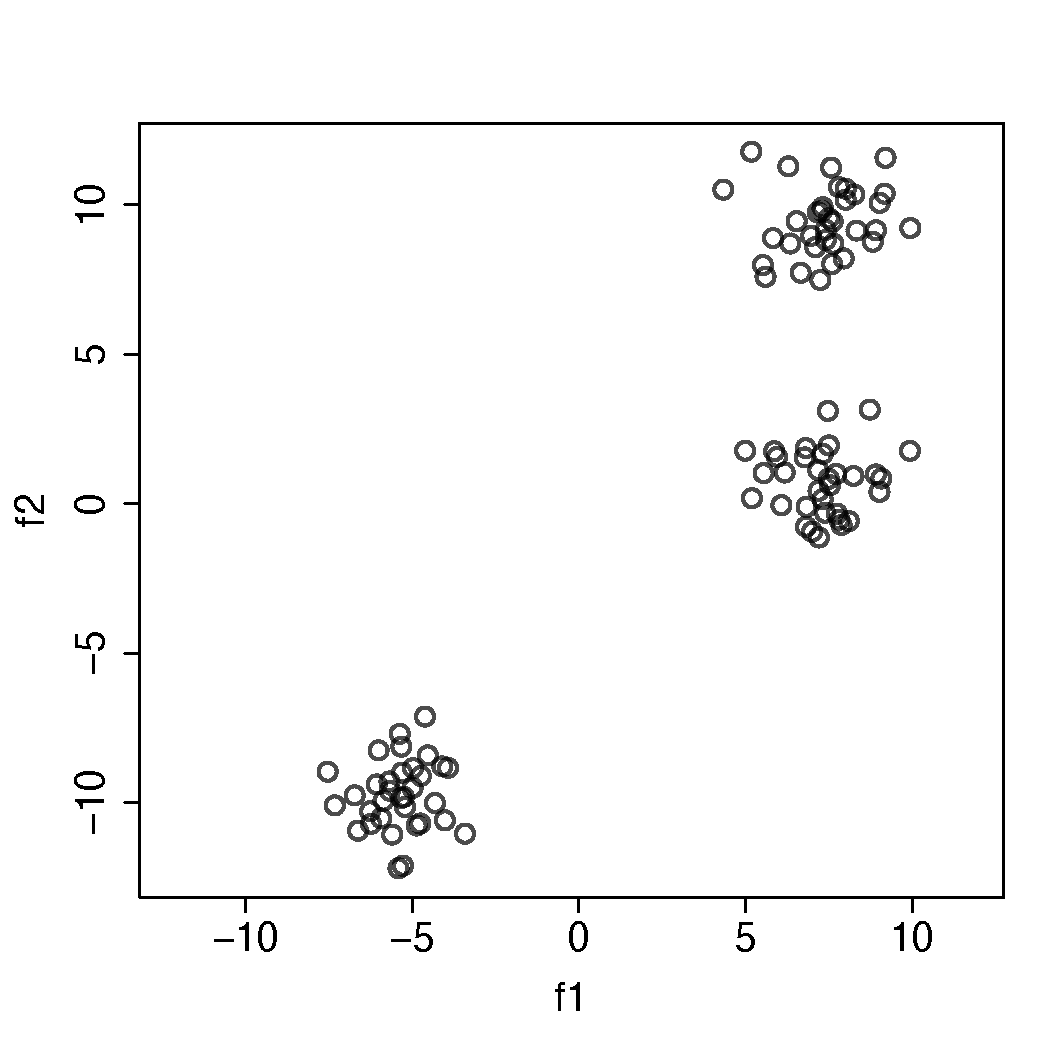
\includegraphics[width=0.333\linewidth]{./images/fmlpda_figure_10_10_a.pdf}} &
	\subfigure[k-means]{\label{fig:blobsKmeans}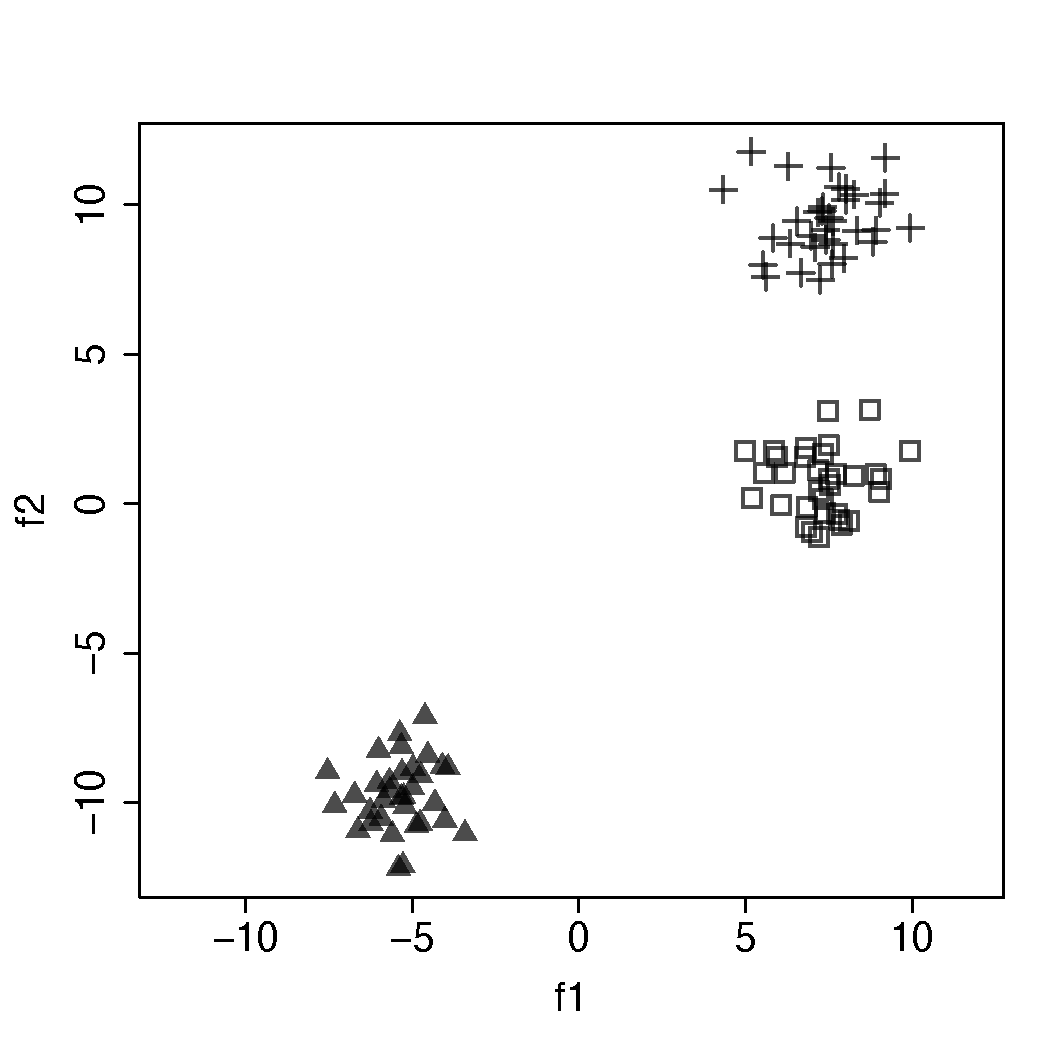
\includegraphics[width=0.333\linewidth]{./images/fmlpda_figure_10_10_b.pdf}}&
	\subfigure[AHC]{\label{fig:blobsAHC}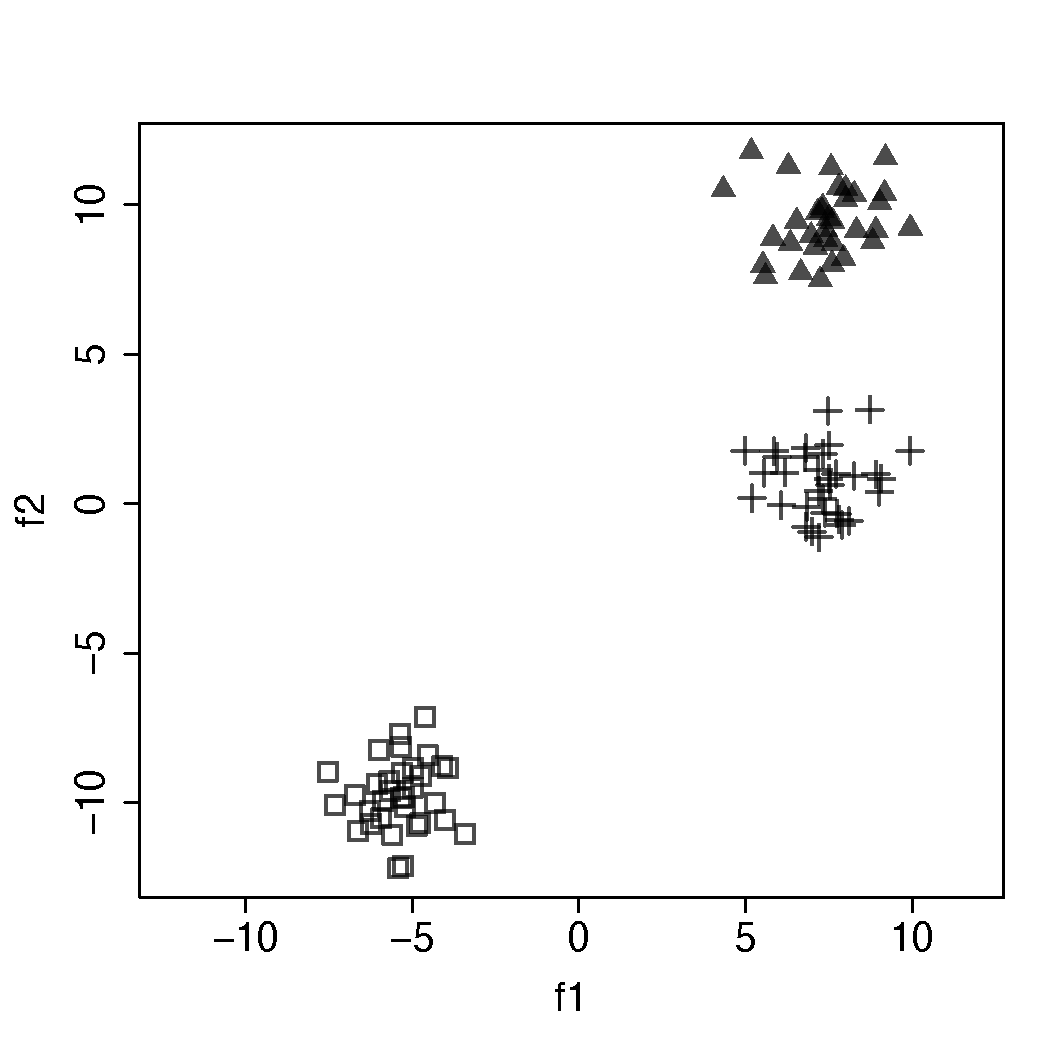
\includegraphics[width=0.333\linewidth]{./images/fmlpda_figure_10_10_c.pdf}} \\	
\end{tabular}
}	
\caption{(a)--(i) A plot of the \textit{blobs}, \textit{circles}, and \textit{half-moons} datasets and the clusterings achieved by the \textit{k}-means clustering and agglomerative hierarchical clustering algorithms (where $k$ is  set to $3$, $2$, and $2$, respectively).}
\label{fig:blobsCirclesMoonsDemo}
\end{figure}
\end{frame} 

 \begin{frame}
 \addtocounter{subfigure}{3}
\begin{figure}[htb]
{\setlength{\tabcolsep}{0.05em}
\begin{tabular}{ccc}
	\subfigure[Circles Dataset]{\label{fig:cirlcesData}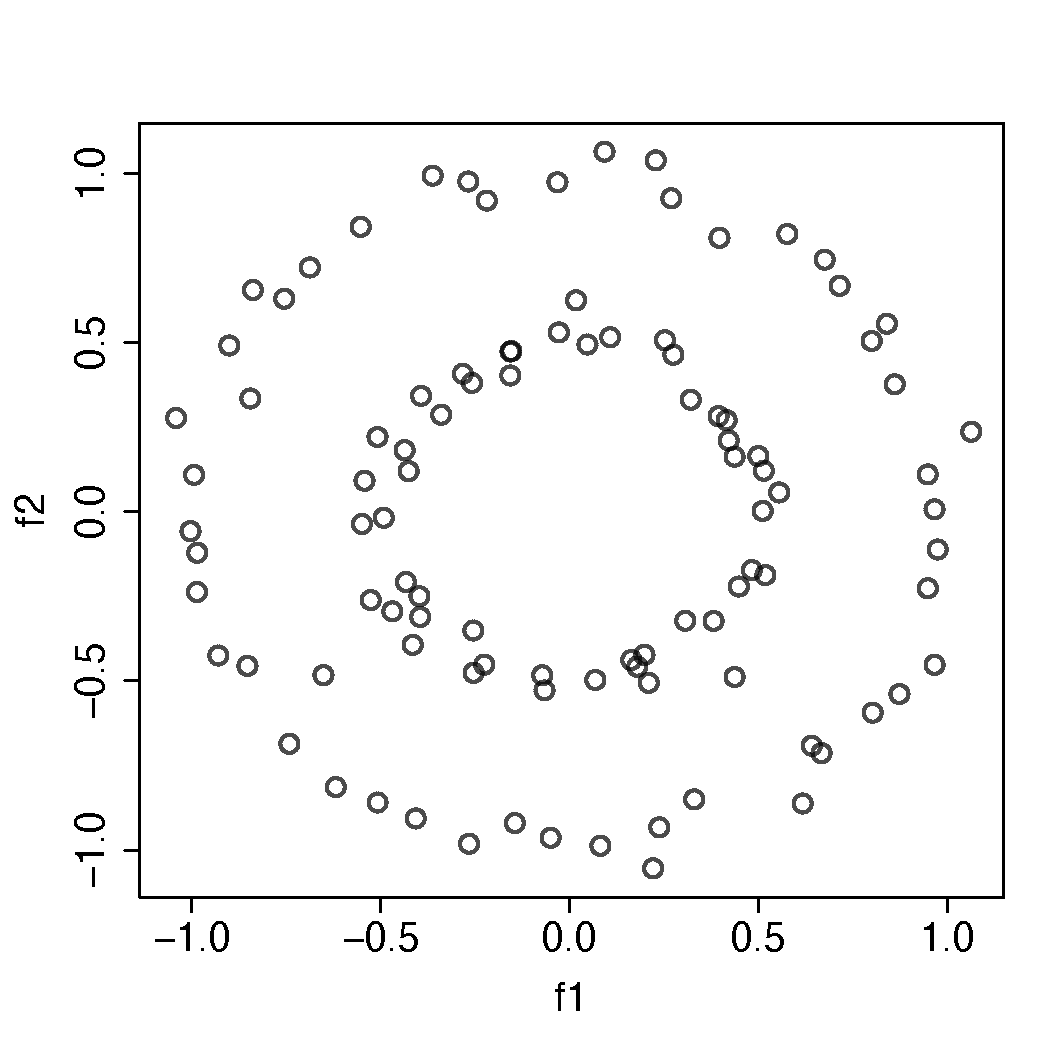
\includegraphics[width=0.333\linewidth]{./images/fmlpda_figure_10_10_d.pdf}}&
	\subfigure[k-means]{\label{fig:cirlcesKmeans}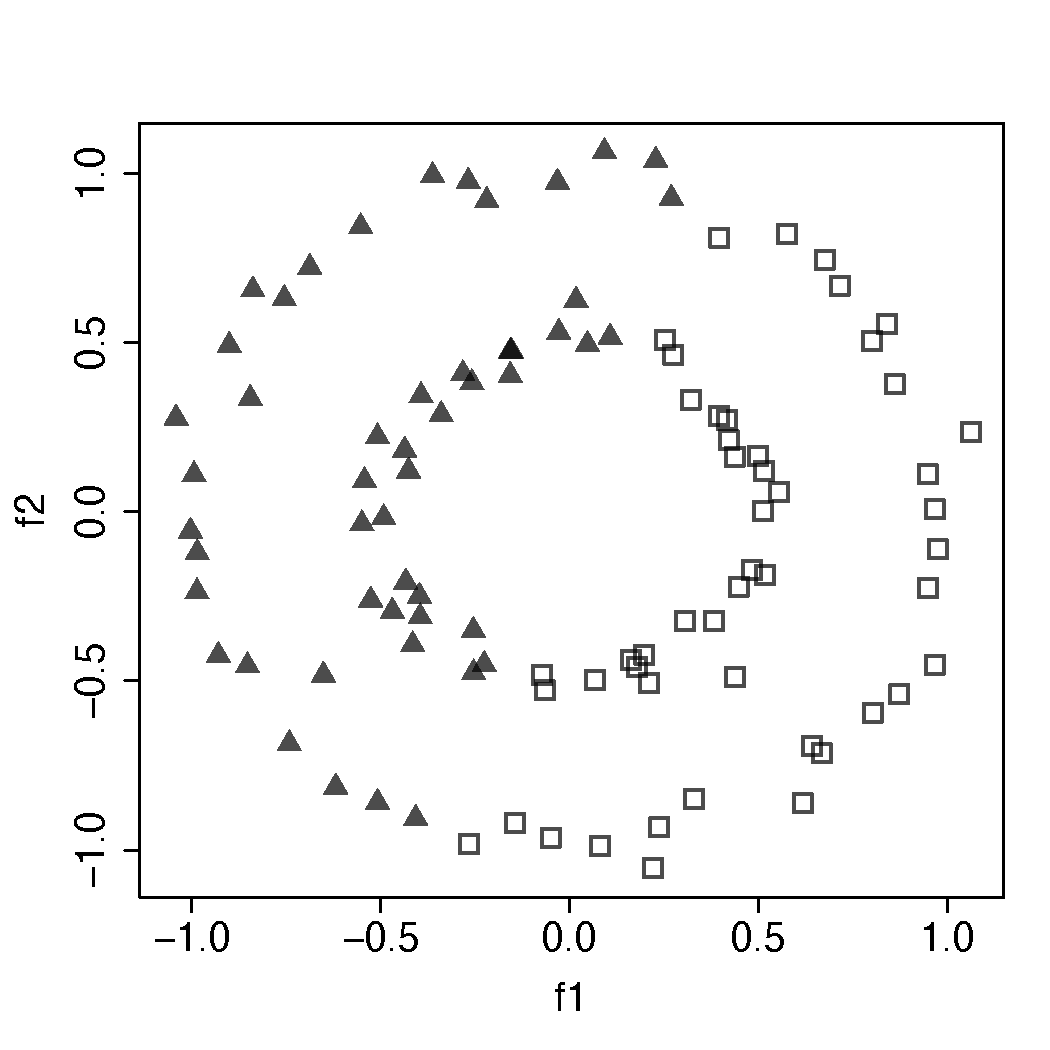
\includegraphics[width=0.333\linewidth]{./images/fmlpda_figure_10_10_e.pdf}}&
	\subfigure[AHC]{\label{fig:cirlcesAHC}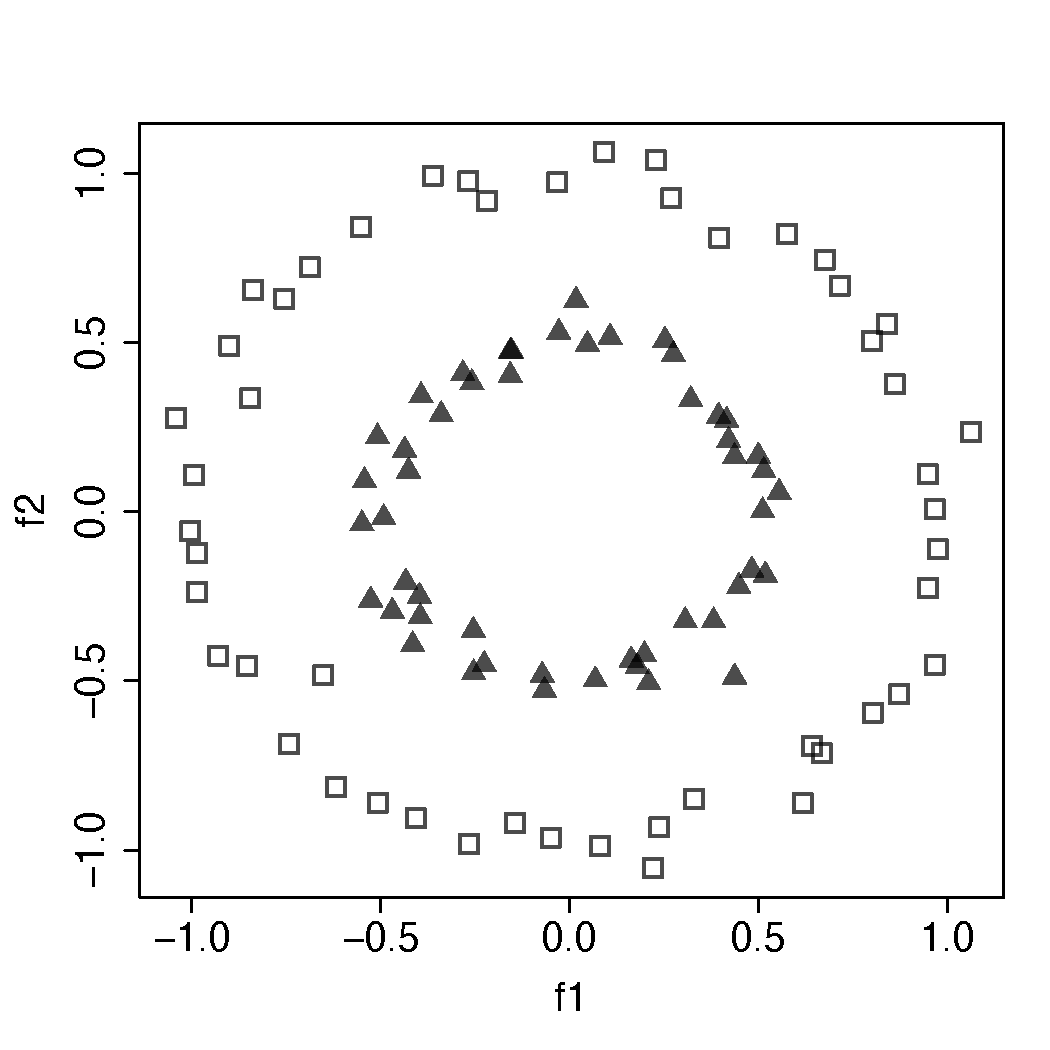
\includegraphics[width=0.333\linewidth]{./images/fmlpda_figure_10_10_f.pdf}} \\	
\end{tabular}
}	
\caption{(a)--(i) A plot of the \textit{blobs}, \textit{circles}, and \textit{half-moons} datasets and the clusterings achieved by the \textit{k}-means clustering and agglomerative hierarchical clustering algorithms (where $k$ is  set to $3$, $2$, and $2$, respectively).}
\label{fig:blobsCirclesMoonsDemo}
\end{figure}
\end{frame} 

 \begin{frame}
  \addtocounter{subfigure}{6}
\begin{figure}[htb]
{\setlength{\tabcolsep}{0.05em}
\begin{tabular}{ccc}
	\subfigure[Half-moons Dataset]{\label{fig:moonsData}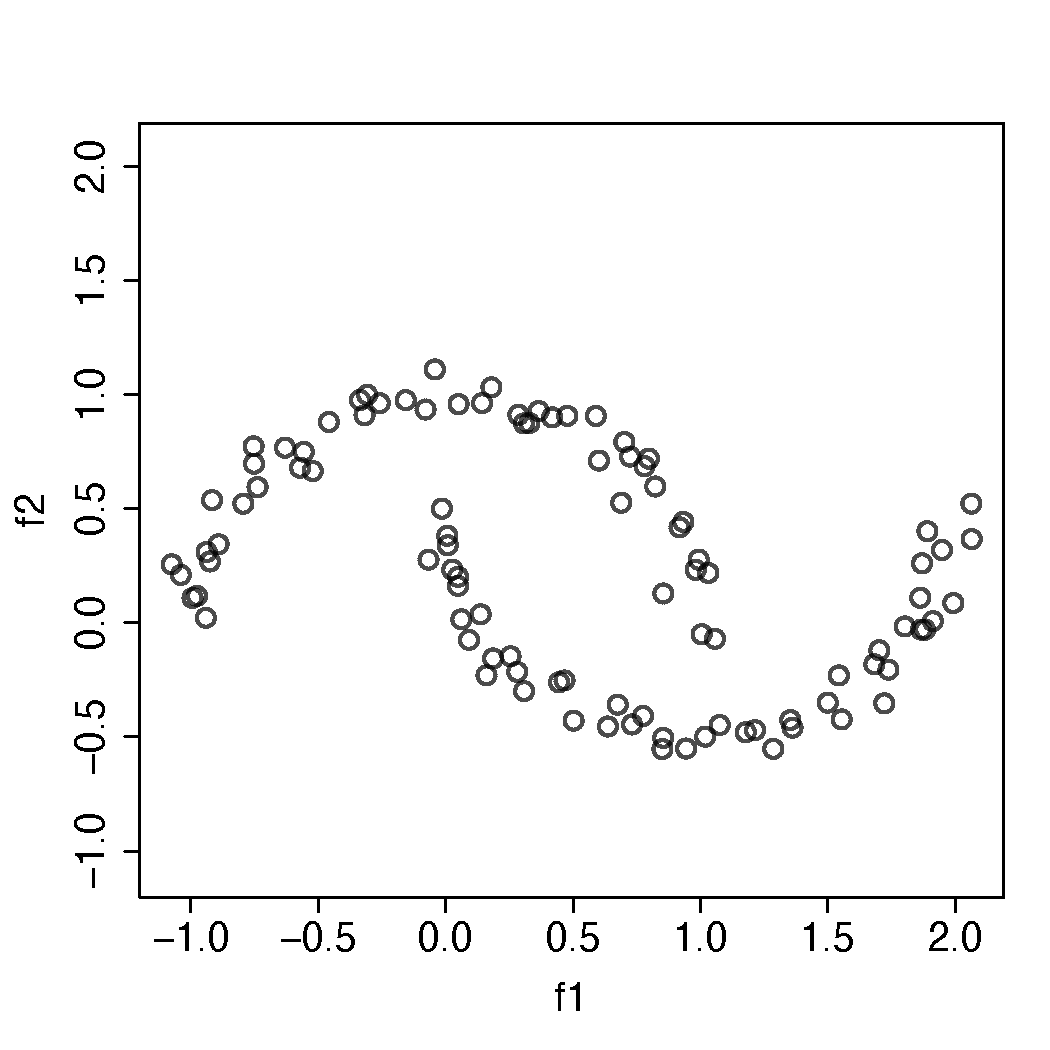
\includegraphics[width=0.333\linewidth]{./images/fmlpda_figure_10_10_g.pdf}}&
	\subfigure[k-means]{\label{moonsKmeans}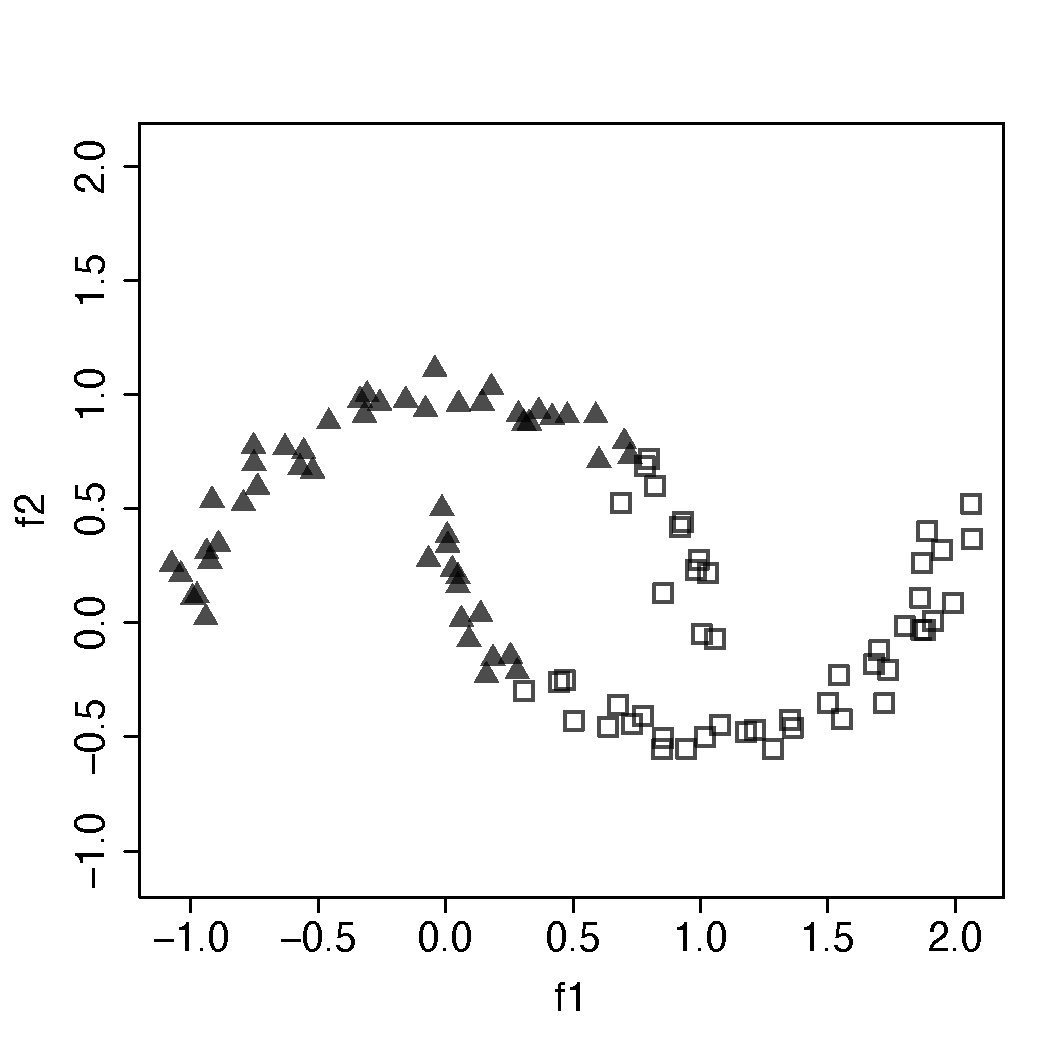
\includegraphics[width=0.333\linewidth]{./images/fmlpda_figure_10_10_h.pdf}} &
	\subfigure[AHC]{\label{fig:moonsAHC}\includegraphics[width=0.333\linewidth]{./images/fmlpda_figure_10_10_i.pdf}} \\
\end{tabular}
}	
\caption{(a)--(i) A plot of the \textit{blobs}, \textit{circles}, and \textit{half-moons} datasets and the clusterings achieved by the \textit{k}-means clustering and agglomerative hierarchical clustering algorithms (where $k$ is  set to $3$, $2$, and $2$, respectively).}
\label{fig:blobsCirclesMoonsDemo}
\end{figure}
\end{frame} 


\begin{frame}[plain]
\scriptsize{Pseudocode description of the \keyword{agglomerative hierarchical clustering} algorithm.}
\begin{footnotesize}
%\begin{algorithm}[htb]
%\caption{Pseudocode description of the \keyword{agglomerative hierarchical clustering} algorithm.}
%\label{alg:ahc}
\begin{algorithmic}[1]
\Require a dataset $\mathcal{D}$ containing $n$ training instances, $\mathbf{d}_1, \ldots, \mathbf{d}_n$ 
\Require a distance measure, ${Dist}$, to compare distances between instances 
\Require a linkage method, $\mathcal{L}$, to compare distances between clusters
\State initialize the hierarchy level, $h=1$
\State divide $\mathcal{D}$ into a set of $n$ disjoint clusters, $\mathbf{\mathcal{C}} = \left\{\mathcal{C}_{1}, \ldots,\mathcal{C}_{n}\right\}$, with one instance in each cluster
\Repeat
\State{using distance measure ${Dist}$ and linkage method $\mathcal{L}$, find the nearest pair of clusters, $\mathcal{C}_{i}$ and $\mathcal{C}_{j}$, in the current clustering}
\State merge $\mathcal{C}_{i}$ and $\mathcal{C}_{j}$ to form a new cluster $\mathcal{C}_{n+h}$
\State remove the old clusters from the clustering: $\mathbf{\mathcal{C}} \leftarrow \mathbf{\mathcal{C}} ~\setminus \left\{\mathcal{C}_{i}, \mathcal{C}_{j}\right\}$ 
\State add the new cluster to the clustering: $\mathbf{\mathcal{C}} \leftarrow \mathbf{\mathcal{C}} \cup \mathcal{C}_{n+h}$ 
\State $h \leftarrow h + 1$
\Until all the instances join into a single cluster 
\end{algorithmic}
%\end{algorithm}
\end{footnotesize}
\end{frame}






 \begin{frame} 
\begin{figure}[htb]
{\setlength{\tabcolsep}{0.05em}
\begin{center}
\begin{tabular}{cc}
	\subfigure[single]{\label{fig:linkageSingle}\includegraphics[width=0.26\textwidth]{./images/fmlpda_figure_10_11_a.pdf}} &
	\subfigure[complete]{\label{fig:linkageComplete}\includegraphics[width=0.26\textwidth]{./images/fmlpda_figure_10_11_b.pdf}} \\
	\subfigure[centroid]{\label{fig:linkageCentroid}\includegraphics[width=0.26\textwidth]{./images/fmlpda_figure_10_11_c.pdf}} &
	\subfigure[average]{\label{fig:linkageAverage}\includegraphics[width=0.26\textwidth]{./images/fmlpda_figure_10_11_d.pdf}} \\
\end{tabular}
\end{center}
}	
\caption{(a)--(d) Different linkage methods that can be used to compare the distances between clusters in agglomerative hierarchical clustering. (Arrows for only some indicative distances are shown in the average linkage diagram (d).)}
\label{fig:linkagemethods}
\end{figure}
\end{frame} 



 \begin{frame} 
\begin{table}[!t]
\caption{\keywordAlias{Distance matrices}{distance matrix} that detail the first three iterations of the AHC algorithm applied to the reduced version of the mobile phone customer dataset in Table \ourRef{table:kmeansDemoData}.}
\label{table:ahcDemoSmallData}
\begin{tiny}
\begin{tabular}{ll}
\subtable[A distance matrix for the instances in the dataset.]{\label{table:ahcDemoSmallDataDist}
{\setlength{\tabcolsep}{0.2em}
\begin{tabular*}{12pc}{@{\extracolsep{\fill}} rrrrrrrrrr @{}}
  \Toprule
 & $d_{4}$ & $d_{15}$ & $d_{8}$ & $d_{11}$ & $d_{5}$ & $d_{19}$ & $d_{24}$ & $d_{7}$ & $d_{23}$ \\ 
  \Midrule
$d_{4}$ & 0.00 &  &  &  &  &  &  &  &  \\ 
  $d_{15}$ & 0.28 & 0.00 &  &  &  &  &  &  &  \\ 
  $d_{8}$ & 0.28 & 0.06 & 0.00 &  &  &  &  &  &  \\ 
  $d_{11}$ & 2.12 & 1.89 & 1.94 & 0.00 &  &  &  &  &  \\ 
  $d_{5}$ & 2.25 & 2.02 & 2.06 & 0.18 & 0.00 &  &  &  &  \\ 
  $d_{19}$ & 2.19 & 1.95 & 2.00 & 0.16 & 0.07 & 0.00 &  &  &  \\ 
  $d_{24}$ & 1.66 & 1.39 & 1.42 & 0.81 & 0.83 & 0.76 & 0.00 &  &  \\ 
  $d_{7}$ & 1.84 & 1.56 & 1.58 & 0.96 & 0.94 & 0.89 & 0.27 & 0.00 &  \\ 
  $d_{23}$ & 1.79 & 1.51 & 1.53 & 1.08 & 1.06 & 1.00 & 0.33 & 0.12 & 0.00 \\ 
   \Botrule
\end{tabular*}
}
}

& 
\subtable[The distance matrix after one iteration of AHC.]{\label{table:ahcDemoSmallDataIter1Dist}
{\setlength{\tabcolsep}{0.2em}
\begin{tabular*}{12pc}{@{\extracolsep{\fill}} rrrrrrrrr @{}}
  \Toprule
 & $d_{4}$ & $~~~~~~~~~\mathcal{C}_{10}$ & $d_{11}$ & $d_{5}$ & $d_{19}$ & $d_{24}$ & $d_{7}$ & $d_{23}$ \\ 
  \Midrule
$d_{4}$ & 0.00 &  &  &  &  &  &  &  \\ 
\multirow[t]{2}{*}{$\mathcal{C}_{10}$} & \multirow[t]{2}{*}{0.28} & \multirow[t]{2}{*}{0.00}  &  &  &  &  &  &  \\ 
   &  &  &  &  &  &  &  &  \\ 
  $d_{11}$ & 2.12 & 1.89 & 0.00 &  &  &  &  &  \\ 
  $d_{5}$ & 2.25 & 2.02 & 0.18 & 0.00 &  &  &  &  \\ 
  $d_{19}$ & 2.19 & 1.95 & 0.16 & 0.07 & 0.00 &  &  &  \\ 
  $d_{24}$ & 1.66 & 1.39 & 0.81 & 0.83 & 0.76 & 0.00 &  &  \\ 
  $d_{7}$ & 1.84 & 1.56 & 0.96 & 0.94 & 0.89 & 0.27 & 0.00 &  \\ 
  $d_{23}$ & 1.79 & 1.51 & 1.08 & 1.06 & 1.00 & 0.33 & 0.12 & 0.00 \\ 
   \Botrule
\end{tabular*}
}
}   \\
\end{tabular}
\end{tiny}
\end{table}
\end{frame} 


 \begin{frame} 
\begin{table}[!t]
\caption{\keywordAlias{Distance matrices}{distance matrix} that detail the first three iterations of the AHC algorithm applied to the reduced version of the mobile phone customer dataset in Table \ourRef{table:kmeansDemoData}.}
\label{table:ahcDemoSmallData}
\begin{tiny}
\begin{tabular}{ll}
   \addtocounter{subtable}{2}
\subtable[The distance matrix after two iterations of AHC.]{\label{table:ahcDemoSmallDataIter3Dist}
{\setlength{\tabcolsep}{0.2em}
\begin{tabular*}{12pc}{@{\extracolsep{\fill}} rrrrrrr @{}}
  \Toprule
	&	$d_{4}$	&	$~~~~~~~~~\mathcal{C}_{10}$	&	$d_{11}$	&	$~~~~~~~~~\mathcal{C}_{11}$	&	$d_{24}$	&	$~~~~~~~~~\mathcal{C}_{12}$	\\
  \Midrule
$d_{4}$	&	0.00	&		&		&		&		&		\\
\multirow[t]{2}{*}{$\mathcal{C}_{10}$}	&	\multirow[t]{2}{*}{0.28}	&	\multirow[t]{2}{*}{0.00}	&		&		&		&		\\
	&	&		&		&		&		&		\\
$d_{11}$	&	2.12	&	1.89	&	0.00	&		&		&		\\
\multirow[t]{2}{*}{$\mathcal{C}_{11}$}	&	\multirow[t]{2}{*}{2.19}	&	\multirow[t]{2}{*}{1.95}	&	\multirow[t]{2}{*}{0.16}	&	\multirow[t]{2}{*}{0.00}	&		&		\\
	&	&		&		&		&		&		\\
$d_{24}$	&	1.66	&	1.39	&	0.81	&	0.76	&	0.00	&		\\
\multirow[t]{2}{*}{$\mathcal{C}_{12}$}	&	\multirow[t]{2}{*}{1.79}	&	\multirow[t]{2}{*}{1.51}	&	\multirow[t]{2}{*}{0.97}	&	\multirow[t]{2}{*}{0.89}	&	\multirow[t]{2}{*}{0.27}	&	\multirow[t]{2}{*}{0.00}	\\   
	&	&		&		&		&		&		\\
   \Botrule
\end{tabular*}
}
{}
}

& 
\subtable[The distance matrix after three iterations of AHC.]{\label{table:ahcDemoSmallDataIter4Dist}
{\setlength{\tabcolsep}{0.2em}
\begin{tabular*}{12pc}{@{\extracolsep{\fill}} rrrrrrr @{}}
  \Toprule
	&	$d_{4}$	&	$~~~~~~~~~~~~~~~~~~\mathcal{C}_{13}$	&	$~~~~~~~~~\mathcal{C}_{11}$	&	$d_{24}$	&	$~~~~~~~~~\mathcal{C}_{12}$	\\
  \Midrule
$d_{4}$	&	0.00	&		&		&		&		\\
\multirow[t]{3}{*}{$\mathcal{C}_{13}$}	&	\multirow[t]{3}{*}{0.28}	&	\multirow[t]{3}{*}{0.00}	&		&		&		&		\\
	&	&	&	&	&	\\
	&	&	&	&	&	\\
\multirow[t]{2}{*}{$\mathcal{C}_{11}$}	&	\multirow[t]{2}{*}{2.19}	&	\multirow[t]{2}{*}{0.16}	&	\multirow[t]{2}{*}{0.00}	&		&		\\
	&	&	&	&	&	\\
$d_{24}$	&	1.66	&	0.81	&	0.76	&	0.00	&		\\
\multirow[t]{2}{*}{$\mathcal{C}_{12}$}	&	\multirow[t]{2}{*}{1.79}	&	\multirow[t]{2}{*}{0.97}	&	\multirow[t]{2}{*}{0.89}	&	\multirow[t]{2}{*}{0.27}	&	\multirow[t]{2}{*}{0.00}	\\   
	&	&	&	&	&	\\
   \Botrule
\end{tabular*}
}
{}
}
\end{tabular}
\end{tiny}
\end{table}
\end{frame} 



 \begin{frame}
\begin{figure}[!t]
{\setlength{\tabcolsep}{0.05em}
\begin{tabular}{ccc}

	\subfigure[]{\label{fig:ahcDemoDataSmall}\includegraphics[width=0.3\linewidth]{./images/fmlpda_figure_10_12_a.pdf}}  &

	\subfigure[]{\label{fig:ahcDemoDataSmallClust1}\includegraphics[width=0.3\linewidth]{./images/fmlpda_figure_10_12_b.pdf}} &

	\subfigure[]{\label{fig:ahcDemoDataSmallClust3}\includegraphics[width=0.3\linewidth]{./images/fmlpda_figure_10_12_c.pdf}} \\

\end{tabular}
}	
\caption[(a) A plot of a reduced version of the mobile phone customer dataset given in Table \ourRef{table:kmeansDemoData}. (b)--(d) show details of several iterations of the AHC algorithm.]{(a) A plot of a reduced version of the mobile phone customer dataset given in Table \ourRef{table:kmeansDemoData}. (b) At the first iteration of the AHC algorithm the first pair of instances is combined into a cluster, $\mathcal{C}_{10}$. (c) After three iterations of the AHC algorithm, three pairs of instances have been combined into clusters, $\mathcal{C}_{10}$, $\mathcal{C}_{11}$, and $\mathcal{C}_{12}$. (d) At the fourth iteration of AHC, the first hierarchical cluster combination is created when a single instance, $d_{11}$ is combined with the cluster $\mathcal{C}_{10}$ to create a new cluster, $\mathcal{C}_{13}$.}
\label{fig:ahcDemo}
\end{figure}
\end{frame} 


\begin{frame}
\addtocounter{subfigure}{3}
\begin{figure}[!t]
{\setlength{\tabcolsep}{0.05em}
\begin{tabular}{ccc}
	\subfigure[]{\label{fig:ahcDemoDataSmallClust4}\includegraphics[width=0.3\linewidth]{./images/fmlpda_figure_10_12_d.pdf}} &
	 
	\subfigure[]{\label{fig:ahcDemoDataSmallClust8}\includegraphics[width=0.3\linewidth]{./images/fmlpda_figure_10_12_e.pdf}}  &

	\subfigure[]{\label{fig:ahcDemoDataSmallTree}\raisebox{20pt}{\includegraphics[width=0.3\linewidth]{./images/fmlpda_figure_10_12_f.pdf}}}  \\ 
\end{tabular}
}	
\caption[(a) A plot of a reduced version of the mobile phone customer dataset given in Table \ourRef{table:kmeansDemoData}. (b)--(d) show details of several iterations of the AHC algorithm.]{(a) A plot of a reduced version of the mobile phone customer dataset given in Table \ourRef{table:kmeansDemoData}. (b) At the first iteration of the AHC algorithm the first pair of instances is combined into a cluster, $\mathcal{C}_{10}$. (c) After three iterations of the AHC algorithm, three pairs of instances have been combined into clusters, $\mathcal{C}_{10}$, $\mathcal{C}_{11}$, and $\mathcal{C}_{12}$. (d) At the fourth iteration of AHC, the first hierarchical cluster combination is created when a single instance, $d_{11}$ is combined with the cluster $\mathcal{C}_{10}$ to create a new cluster, $\mathcal{C}_{13}$.}
\label{fig:ahcDemo}
\end{figure}
\end{frame} 

 \begin{frame} 
 \begin{figure}[!htb]
 \vspace{-20pt}
{\setlength{\tabcolsep}{0.05em}
\begin{center}
\begin{tabular}{l}

	\subfigure[AHC result]{\label{fig:ahcTree}\includegraphics[width=0.6\linewidth]{./images/fmlpda_figure_10_13_a.pdf}}  \\
		
\end{tabular}
\end{center}
}	
\caption{(a) A plot of the hierarchical grouping of the instances in the mobile phone customer dataset from Table \ourRef{table:kmeansDemoData} found by the AHC algorithm (using Euclidean distance and single linkage). (b) The clustering returned when the tree is cut at $k=3$. (c) The clustering returned when the tree is cut at $k=6$.}
\label{fig:ahcPhonesDemo}
\end{figure}
\end{frame} 


 \begin{frame} 
 \addtocounter{subfigure}{1}
 \begin{figure}[!htb]
 \vspace{-20pt}
{\setlength{\tabcolsep}{0.05em}
\begin{center}
\begin{tabular}{l}
		 
	\subfigure[Clustering cut at $k=3$]{\label{fig:ahcTreeCut3}\includegraphics[width=0.6\linewidth]{./images/fmlpda_figure_10_13_b_i.pdf}~\includegraphics[width=0.36\linewidth]{./images/fmlpda_figure_10_13_b_ii.pdf}} \\
		
\end{tabular}
\end{center}
}	
\caption{(a) A plot of the hierarchical grouping of the instances in the mobile phone customer dataset from Table \ourRef{table:kmeansDemoData} found by the AHC algorithm (using Euclidean distance and single linkage). (b) The clustering returned when the tree is cut at $k=3$. (c) The clustering returned when the tree is cut at $k=6$.}
\label{fig:ahcPhonesDemo}
\end{figure}
\end{frame} 

 \begin{frame} 
  \addtocounter{subfigure}{2}
 \begin{figure}[!htb]
 \vspace{-20pt}
{\setlength{\tabcolsep}{0.05em}
\begin{center}
\begin{tabular}{l}

	\subfigure[Clustering cut at $k=6$]{\label{fig:ahcTreeCut6}\includegraphics[width=0.6\linewidth]{./images/fmlpda_figure_10_13_c_i.pdf}~\includegraphics[width=0.36\linewidth]{./images/fmlpda_figure_10_13_c_ii.pdf}} \\
		
\end{tabular}
\end{center}
}	
\caption{(a) A plot of the hierarchical grouping of the instances in the mobile phone customer dataset from Table \ourRef{table:kmeansDemoData} found by the AHC algorithm (using Euclidean distance and single linkage). (b) The clustering returned when the tree is cut at $k=3$. (c) The clustering returned when the tree is cut at $k=6$.}
\label{fig:ahcPhonesDemo}
\end{figure}
\end{frame} 


\subsection{Representation Learning with Auto-Encoders}



 \begin{frame} 
\begin{figure}[htb]
       \begin{centering}
       \includegraphics[width=0.85\textwidth]{images/fmlpda_figure_10_14.pdf}
       \caption{The architecture of an auto-encoder network made up of an encoder and a decoder connected by a bottleneck layer.}.
       \label{fig:autoencoder_architecture}
       \end{centering}
\end{figure}
\end{frame} 



 \begin{frame} [plain]
\begin{figure}[!tbh]
\begin{center}
	\subfigure[]{\label{fig:digits_original}{\setlength{\tabcolsep}{0.05em}
\begin{tabular}{ccccccccc}
\includegraphics[width=0.08\textwidth]{./images/fmlpda_figure_10_15_a_i.pdf} &
\includegraphics[width=0.08\textwidth]{./images/fmlpda_figure_10_15_a_ii.pdf} &
\includegraphics[width=0.08\textwidth]{./images/fmlpda_figure_10_15_a_iii.pdf} &
\includegraphics[width=0.08\textwidth]{./images/fmlpda_figure_10_15_a_iv.pdf} &
\includegraphics[width=0.08\textwidth]{./images/fmlpda_figure_10_15_a_v.pdf} &
\includegraphics[width=0.08\textwidth]{./images/fmlpda_figure_10_15_a_vi.pdf} &
\includegraphics[width=0.08\textwidth]{./images/fmlpda_figure_10_15_a_vii.pdf} &
\includegraphics[width=0.08\textwidth]{./images/fmlpda_figure_10_15_a_viii.pdf} &
\includegraphics[width=0.08\textwidth]{./images/fmlpda_figure_10_15_a_ix.pdf} \\

	\end{tabular}
}}

	\subfigure[]{\label{fig:digits_0_training}{\setlength{\tabcolsep}{0.05em}
\begin{tabular}{ccccccccc}
\includegraphics[width=0.08\textwidth]{./images/fmlpda_figure_10_15_b_i.pdf} &
\includegraphics[width=0.08\textwidth]{./images/fmlpda_figure_10_15_b_ii.pdf} &
\includegraphics[width=0.08\textwidth]{./images/fmlpda_figure_10_15_b_iii.pdf} &
\includegraphics[width=0.08\textwidth]{./images/fmlpda_figure_10_15_b_iv.pdf} &
\includegraphics[width=0.08\textwidth]{./images/fmlpda_figure_10_15_b_v.pdf} &
\includegraphics[width=0.08\textwidth]{./images/fmlpda_figure_10_15_b_vi.pdf} &
\includegraphics[width=0.08\textwidth]{./images/fmlpda_figure_10_15_b_vii.pdf} &
\includegraphics[width=0.08\textwidth]{./images/fmlpda_figure_10_15_b_viii.pdf} &
\includegraphics[width=0.08\textwidth]{./images/fmlpda_figure_10_15_b_ix.pdf} \\

	\end{tabular}
}}
	\subfigure[]{\label{fig:digits_5_training}{\setlength{\tabcolsep}{0.05em}
\begin{tabular}{ccccccccc}
\includegraphics[width=0.08\textwidth]{./images/fmlpda_figure_10_15_c_i.pdf} &
\includegraphics[width=0.08\textwidth]{./images/fmlpda_figure_10_15_c_ii.pdf} &
\includegraphics[width=0.08\textwidth]{./images/fmlpda_figure_10_15_c_iii.pdf} &
\includegraphics[width=0.08\textwidth]{./images/fmlpda_figure_10_15_c_iv.pdf} &
\includegraphics[width=0.08\textwidth]{./images/fmlpda_figure_10_15_c_v.pdf} &
\includegraphics[width=0.08\textwidth]{./images/fmlpda_figure_10_15_c_vi.pdf} &
\includegraphics[width=0.08\textwidth]{./images/fmlpda_figure_10_15_c_vii.pdf} &
\includegraphics[width=0.08\textwidth]{./images/fmlpda_figure_10_15_c_viii.pdf} &
\includegraphics[width=0.08\textwidth]{./images/fmlpda_figure_10_15_c_ix.pdf} \\

	\end{tabular}
}}

	\subfigure[]{\label{fig:digits_300_training}{\setlength{\tabcolsep}{0.05em}
\begin{tabular}{ccccccccc}
\includegraphics[width=0.08\textwidth]{./images/fmlpda_figure_10_15_d_i.pdf} &
\includegraphics[width=0.08\textwidth]{./images/fmlpda_figure_10_15_d_ii.pdf} &
\includegraphics[width=0.08\textwidth]{./images/fmlpda_figure_10_15_d_iii.pdf} &
\includegraphics[width=0.08\textwidth]{./images/fmlpda_figure_10_15_d_iv.pdf} &
\includegraphics[width=0.08\textwidth]{./images/fmlpda_figure_10_15_d_v.pdf} &
\includegraphics[width=0.08\textwidth]{./images/fmlpda_figure_10_15_d_vi.pdf} &
\includegraphics[width=0.08\textwidth]{./images/fmlpda_figure_10_15_d_vii.pdf} &
\includegraphics[width=0.08\textwidth]{./images/fmlpda_figure_10_15_d_viii.pdf} &
\includegraphics[width=0.08\textwidth]{./images/fmlpda_figure_10_15_d_ix.pdf} \\

	\end{tabular}
}}
\end{center}
\caption[(a) A selection of images from the handwritten digits dataset; (b)--(d) image reconstructions generated by the auto-encoder network after $0$, $10$, and $1{,}000$ training epochs.]{(a) A selection of images from the handwritten digits dataset; (b) image reconstructions generated by the auto-encoder network before training; (c) image reconstructions generated by the auto-encoder network after minimal training ($10$ epochs); and (d) image reconstructions generated by the auto-encoder network after complete training ($1{,}000$ epochs).}
\label{fig:mnist_original}
\end{figure}
\end{frame} 



 \begin{frame}[plain]
\begin{figure}[!b]
{\setlength{\tabcolsep}{0.05em}
\begin{tiny}
\begin{tabular}[t]{rccr}
\textbf{Training} & \textbf{Image} & \textbf{Pixel Values} & \textbf{Error} \\
~ & ~ & ~ & ~\\
Original& \includegraphics[width=0.15\textwidth, valign = c]{./images/fmlpda_figure_10_16_i.pdf} &
\begin{scriptsize}$\begin{bmatrix}
  0.00 &   0.19 &   0.94 &   1.00 &   0.88 &   0.06 &   0.00 &   0.00\\
  0.00 &   0.12 &   0.75 &   0.81 &   1.00 &   0.25 &   0.00 &   0.00\\
  0.00 &   0.00 &   0.00 &   0.38 &   1.00 &   0.19 &   0.00 &   0.00\\
  0.00 &   0.00 &   0.06 &   0.94 &   0.62 &   0.00 &   0.00 &   0.00\\
  0.00 &   0.00 &   0.38 &   1.00 &   0.25 &   0.00 &   0.00 &   0.00\\
  0.00 &   0.12 &   0.94 &   0.62 &   0.00 &   0.00 &   0.00 &   0.00\\
  0.00 &   0.25 &   1.00 &   0.69 &   0.50 &   0.69 &   0.19 &   0.00\\
  0.00 &   0.19 &   1.00 &   1.00 &   1.00 &   0.75 &   0.19 &   0.00\\
  \end{bmatrix}$\end{scriptsize}&
$~~~~~~$ \\ 
~ & ~ & ~& ~  \\
0~Epochs & \includegraphics[width=0.15\textwidth, valign = c]{./images/fmlpda_figure_10_16_ii.pdf} &
\begin{scriptsize}~$\begin{bmatrix}
  0.51 &   0.48 &   0.49 &   0.49 &   0.51 &   0.50 &   0.49 &   0.50\\
  0.51 &   0.50 &   0.49 &   0.52 &   0.51 &   0.51 &   0.51 &   0.49\\
  0.51 &   0.52 &   0.50 &   0.51 &   0.50 &   0.49 &   0.52 &   0.50\\
  0.50 &   0.51 &   0.51 &   0.51 &   0.50 &   0.50 &   0.49 &   0.50\\
  0.50 &   0.47 &   0.50 &   0.52 &   0.51 &   0.50 &   0.52 &   0.50\\
  0.51 &   0.51 &   0.50 &   0.49 &   0.53 &   0.50 &   0.51 &   0.49\\
  0.51 &   0.52 &   0.49 &   0.51 &   0.51 &   0.50 &   0.51 &   0.50\\
  0.50 &   0.50 &   0.48 &   0.51 &   0.50 &   0.51 &   0.51 &   0.51\\
\end{bmatrix}$ ~ \end{scriptsize}&
$0.1876$ \\ 
\end{tabular}
\end{tiny}}
\caption{An image of the digit $2$ and reconstructions of this image by the auto-encoder after various amounts of network training. The pixel values of the reconstructed images are shown alongside the images, as is the reconstruction error calculated by comparing these to the pixel values of the original image.}
\label{fig:auto_encoder_reconstruction_errors}
\end{figure}
\end{frame} 


 \begin{frame}[plain]
\begin{figure}[!b]
{\setlength{\tabcolsep}{0.05em}
\begin{tiny}
\begin{tabular}[t]{rccr}
\textbf{Training} & \textbf{Image} & \textbf{Pixel Values} & \textbf{Error} \\
~ & ~ & ~ & ~\\
10~Epochs & \includegraphics[width=0.15\textwidth, valign = c]{./images/fmlpda_figure_10_16_iii.pdf} &
\begin{scriptsize}~$\begin{bmatrix}
  0.00 &   0.00 &   0.42 &   0.83 &   0.76 &   0.33 &   0.03 &   0.00\\
  0.01 &   0.12 &   0.80 &   0.76 &   0.74 &   0.62 &   0.06 &   0.00\\
  0.00 &   0.15 &   0.60 &   0.35 &   0.54 &   0.58 &   0.07 &   0.00\\
  0.00 &   0.09 &   0.49 &   0.57 &   0.68 &   0.46 &   0.11 &   0.00\\
  0.00 &   0.08 &   0.31 &   0.57 &   0.68 &   0.48 &   0.13 &   0.01\\
  0.00 &   0.05 &   0.31 &   0.37 &   0.41 &   0.51 &   0.19 &   0.00\\
  0.00 &   0.02 &   0.49 &   0.59 &   0.59 &   0.63 &   0.21 &   0.01\\
  0.00 &   0.01 &   0.45 &   0.85 &   0.74 &   0.39 &   0.09 &   0.01\\
 \end{bmatrix}$ ~ \end{scriptsize}&
$0.0685$ \\ 
~ & ~ & ~& ~  \\
$1{,}000$ Epochs & \includegraphics[width=0.15\textwidth, valign = c]{./images/fmlpda_figure_10_16_iv.pdf} &
\begin{scriptsize}~$\begin{bmatrix}
  0.00 &   0.06 &   0.71 &   0.87 &   0.71 &   0.10 &   0.00 &   0.00\\
  0.00 &   0.32 &   0.70 &   0.77 &   0.86 &   0.30 &   0.00 &   0.00\\
  0.00 &   0.11 &   0.09 &   0.75 &   0.97 &   0.24 &   0.00 &   0.00\\
  0.00 &   0.00 &   0.00 &   0.86 &   0.93 &   0.08 &   0.00 &   0.00\\
  0.00 &   0.00 &   0.02 &   0.88 &   0.62 &   0.00 &   0.00 &   0.00\\
  0.00 &   0.01 &   0.68 &   0.89 &   0.24 &   0.04 &   0.01 &   0.00\\
  0.00 &   0.32 &   0.91 &   0.89 &   0.53 &   0.51 &   0.19 &   0.00\\
  0.00 &   0.03 &   0.78 &   0.89 &   0.83 &   0.69 &   0.21 &   0.00\\
\end{bmatrix}$ ~ \end{scriptsize}&
$0.0179$ \\ 
\end{tabular}
\end{tiny}}
\caption{An image of the digit $2$ and reconstructions of this image by the auto-encoder after various amounts of network training. The pixel values of the reconstructed images are shown alongside the images, as is the reconstruction error calculated by comparing these to the pixel values of the original image.}
\label{fig:auto_encoder_reconstruction_errors}
\end{figure}
\end{frame} 


 \begin{frame} 
\begin{figure}[htb]
       \begin{centering}
       \includegraphics[width=0.99\textwidth]{images/fmlpda_figure_10_17.pdf}
       \caption{The process of using an unsupervised auto-encoder network to generate a feature representation used to train a supervised model.}
       \label{fig:unsupervised_supervied_process_flow}
       \end{centering}
\end{figure}
\end{frame} 


\SectionSlide{Summary}

\begin{frame}
\begin{itemize}
	\item Unsupervised machine learning techniques are used in the absence of a target feature  and model the underlying structure within the descriptive features in a dataset. W
	\item We can think of the output of most unsupervised machine learning models as new generated features that can be appended to the original dataset to \keywordAlias{augment}{augment data} or \keywordAlias{enrich}{enrich data} it. 
	\item There are two key main use cases for unsupervised learning: clustering and representation learning. 
	\item Two clustering techniques were presented in detail: \keywordAlias{\textit{k}-means clustering}{k-means clustering} and \keyword{agglomerative hierarchical clustering} (AHC). 
\end{itemize}
\end{frame}

\begin{frame}
\begin{itemize}
\item \keywordAlias{Neural network}{neural network} models are especially effective for representation learning, and the chapter presented an example of using an \keyword{auto-encoder} to learn a feature representation that could be used by a supervised machine learning model. 

\item Applications of unsupervised learning are widespread, including customer segmentations, anomaly detection, and analyzing people's movement patterns.

\item Designing solutions based on unsupervised machine learning techniques can be quite creative. 
\item Finally, unsupervised learning is a fascinating research area and has  many significant open research challenges.

\end{itemize}
\end{frame}

\SectionSlide{Further Reading}

\begin{frame}
\begin{itemize}
	\item For more detail on unsupervised machine learning algorithms \citep{friedman2001elements} has a fairly comprehensive unsupervised learning section.
	\item For good treatments of unsupervised learning applications see \citep{berry2004data,han2011data}.
\item \citep{guo2016deep} provides a readable, coherent overview of different types of autoencoder models.
\end{itemize}
\end{frame}

\begin{frame}
	%\tableofcontents
	 \tableofcontents[hideallsubsections]
\end{frame}

%\bibliographystyle{apalike}
\bibliographystyle{./mit-chicago-FMLPDA}
\bibliography{./FMLPDA2Bib_Brian}


\end{document}
